%!TEX root = ../thesis.tex
%*******************************************************************************
%****************************** Sixth Chapter **********************************
%*******************************************************************************

% **************************** Define Graphics Path **************************
\ifpdf
    \graphicspath{{content/chapter7/figs/raster/}{content/chapter7/figs/pdf/}{content/chapter7/figs/}}
\else
    \graphicspath{{content/chapter7/figs/vector/}{content/chapter7/figs/}}
\fi



% \todo{separate nomenclature into matehmatical symbols and climate indices}



\chapter[Shared Variability between Temporally Lagged Sea Surface Temperature and Continental Precipitation]{Shared Variability between Temporally Lagged\\Sea Surface Temperature and Continental Precipitation}\label{chapter:tele}

The Earth's climate system is highly complex, with various components interacting across different spatial and temporal scales. A key aspect of these interactions is atmospheric teleconnections---large-scale patterns of pressure and circulation anomalies that link climate and weather conditions across distant regions, often thousands of kilometers apart. These teleconnections enable climate variations in one area to influence weather and climate in far-reaching locations. For example, the El Niño-Southern Oscillation (ENSO) significantly affects global weather patterns, altering rainfall and temperature distributions far from the Pacific Ocean where it originates \cite{rodriguez-fonseca_review_2016,scaife_enso_2024}. Similarly, the North Atlantic Oscillation (NAO) impacts weather in Europe and North America.

A critical feature of atmospheric teleconnections is their lagged nature; the influence of a climatic anomaly in one region on another does not occur instantaneously but with a temporal delay. For instance, the atmospheric response to ENSO typically manifests several months after the peak of an El Niño event, with the maximum response in the tropical North Atlantic occurring approximately five months later \cite{enfield_tropical_1997,klein_remote_1999,saravanan_interaction_2000}. Understanding these delayed relationships is essential for enhancing the predictability of climate variability, thereby improving climate forecasts from sub-seasonal to decadal timescales \cite{stan_review_2017,yuan_interconnected_2018}. Additionally, incorporating lagged teleconnections into climate models leads to more accurate simulations and projections by accounting for previously unrecognized interactions.

While teleconnections have been extensively studied across various timescales---from intraseasonal \cite[e.g.][]{stan_review_2017,yuan_interconnected_2018} to decadal \cite[e.g.][]{li_tropical_2021}---many studies have employed hypothesis-driven approaches. There is a growing need for data-driven, exploratory analyses that can identify dominant patterns of shared variability without prior assumptions. This chapter addresses this need by examining the shared variability between sea surface temperatures (SST) and continental precipitation across seasonal to decadal timescales. We utilize rotated Hilbert Maximum Covariance Analysis (MCA; see Section~\ref{sec:theory:mca}) to uncover and interpret the dominant patterns of covariability, implicitly capturing lagged teleconnections through the Hilbert transform and enhancing interpretability through mode rotation.

Preliminary results from this research were published in 

\begin{itemize}
    \item \highlightnames{1}{\fullcite{rieger_lagged_2021}},
\end{itemize}

demonstrating the effectiveness of Hilbert MCA in identifying lagged teleconnections between SST and precipitation. This thesis chapter extends those findings in several significant ways. First, it expands the spatial and temporal scope of the analysis by incorporating newly available data. Second, it introduces a more objective method for determining the number of rotated modes, thereby increasing the robustness of the results. Finally, it explores the implications of focusing on correlation instead of covariance as a metric for shared variability, utilizing and extending the Continuous Power Canonical Correlation Analysis (CPCCA) framework introduced by \citet{swenson_continuum_2015}.

The structure of this chapter is as follows: We begin by describing the data sources and methodological framework (Section~\ref{sec:tele:methods}), with a particular focus on the data preprocessing and analysis decisions. Next, we present the results, highlighting the first ten rotated modes of shared variability between SST and continental precipitation (Section~\ref{sec:tele:results}). These findings are then discussed in relation to existing climate indices and known teleconnection patterns, highlighting both consistencies and novel insights. Finally, we conclude with a summary of the key findings and their implications for future climate research and forecasting (Section~\ref{sec:tele:conclusions}).



\section{Methods and Data}\label{sec:tele:methods}

We used the fifth-generation ERA5 reanalysis dataset provided by the European Centre for Medium-Range Weather Forecasts (ECMWF) \cite{c3s_era5_monthly_single} to investigate the shared variability between SST and continental precipitation on seasonal to decadal time scales. ERA5 offers global coverage on a regular longitude-latitude grid with a spatial resolution of \ang{0.25} and monthly temporal resolution. Spanning from 1940 to the present, it allows us to capture long-term climate variability, trends, and potential teleconnections between SST and precipitation. ERA5 has proven to be a reliable source for climate studies due to its high spatial resolution and strong agreement with observations \cite{hersbach_era5_2020, yao_evaluation_2021, soci_era5_2024}. Precipitation is particularly well represented in the extratropics of the Northern Hemisphere, where most continental landmass resides, making it a suitable proxy for observational data. However, the representation of precipitation in the tropics is less accurate \cite{lavers_evaluation_2022}, which we need to consider when discussing dominant patterns of variability in tropical precipitation. Nevertheless, the recent extension of ERA5 back to 1940---which we used here---has significantly improved the representation of precipitation during the 1950s and 1960s \cite{soci_era5_2024}.

Our geographical focus is between \ang{60}S and \ang{70}N because the majority of landmasses experiencing mostly liquid precipitation lie within these latitudes. Excluding Antarctica helped us avoid biases due to its extreme dryness and sparse observational data. Additionally, SST variability is less reliable in polar regions because of partial sea ice coverage throughout the year. The Southern Hemisphere, in general, has historically fewer observations, affecting data reliability \cite{soci_era5_2024}.

We concentrated on continental precipitation by masking out oceanic precipitation using the land-ocean mask at a 1:110 million scale provided by Natural Earth\footnote{\url{naturalearthdata.com}}. To emphasize teleconnections operating on annual to decadal time scales, we applied a centered 7-month moving average to both the SST and precipitation time series. This approach removed high-frequency variability, such as monsoonal circulations, while retaining low-frequency phenomena like ENSO and PDO. Importantly, we retained the seasonal cycle to test whether we can recover dominant modes of variability using rotated Hilbert MCA (see Section~\ref{sec:theory:mca}) despite its presence in the data.

Our study aims to identify teleconnections---connections between SST and continental precipitation in regions that are not necessarily geographically close (Figure~\ref{fig:tele:trends}~A,~B). However, local connections between SST and precipitation are common; for example, coastal precipitation and river plumes are related to changes in SST \cite[e.g.][]{lenderink_intense_2009}. Since ERA5's high spatial resolution (approximately 30 km at the equator) can resolve these processes, it's likely that an MCA of both datasets might also detect these local-scale phenomena. To mitigate the influence of small-scale processes and focus on larger-scale teleconnections, we coarsened the data by applying spatial averaging from a \ang{0.25} to a \ang{1.00} longitude-latitude grid, effectively smoothing out localized patterns. This processing step left us with 36,588 and 16,920 non-masked grid cells (features) for SST and continental precipitation, respectively. Additionally, to counter the effect of grid size distortion toward the poles \cite{north_latitude_1982}, we applied latitude weighting to the data as described in Section~\ref{sec:theory:pca}.

To detect lagged covariance between SST and precipitation, we applied the Hilbert transform to each time series individually, converting them into complex-valued datasets. To minimize boundary effects and spectral leakage caused by the Hilbert transform (see Section~\ref{sec:theory:pca}), we first extended each time series in both directions using an exponential function. This function starts at the initial or final value of the time series and decays towards the overall trend or mean, depending on the presence of a trend in the data, with a characteristic decay time of three months. This method ensures a smooth transition at the boundaries, avoiding abrupt jumps and aligning the decay with the dominant seasonal cycle in the dataset. As a result, each time series became two times longer than its original length. After applying the Hilbert transform to the extended series, we trimmed the extra sections, retaining only the original time series within the complex data. This approach prevents the Hilbert transform from artificially inflating the data's variance, which could lead to spurious correlations in the Hilbert MCA analysis \cite{rieger_lagged_2021}.

Handling the large cross-covariance matrix---in the order of $10^4 \times 10^4$---poses significant computational challenges. To address this, we performed Hilbert MCA in the principal component (PC) space \cite{barnett_origins_1987}. Initially, we transformed each dataset into its principal axes and retained enough principal components to explain \qty{99}{\percent} of the variance in each dataset. This reduction resulted in 74 components for SST and 199 components for continental precipitation, shrinking the cross-covariance matrix to a more manageable size of 74 $\times$ 199. Reducing the dimensionality not only makes the computations feasible but typically also helps stabilizing the solution by regularizing the initially ill-conditioned\footnote{An ill-conditioned problem arises when small perturbations in the input data, such as noise or numerical errors, lead to large changes in the output solution. This sensitivity is quantified by the \textit{condition number} of a matrix $A$, defined as the ratio of its largest to smallest singular value, $\kappa_c = \sigma_{\text{max}}(A) / \sigma_{\text{min}}(A)$. High condition numbers indicate a matrix that is highly sensitive to errors \cite[e.g.][Section 2.6]{golub_matrix_2013}. In our case, the cross-covariance matrix was too large to decompose directly without HPC infrastructure. However, given its size and the near-linear dependencies between variables, it is reasonable to assume a high condition number. By reducing dimensionality using principal components, the latent variables become orthogonal, effectively lowering the condition number and improving numerical stability.} problem \cite{barnett_origins_1987}.

With the dimensionality reduced, we conducted MCA on the Hilbert-complexified, PC-transformed data to identify shared variability patterns between SST and continental precipitation. In the PC space, the total shared variability is represented by 74 modes. Analysis of the squared covariance fraction (SCF) for the initial non-rotated modes (Figure~\ref{fig:tele:singular_spectrum}~A) revealed that nearly all squared covariance is captured within the first six modes, with the SCF dropping below \qty{0.01}{\percent} for subsequent modes. This rapid decline can also be understood by the fact that \emph{squared} covariance is measured. 

To enhance interpretability, we applied an additional rotation to the MCA solution (Section~\ref{sec:theory:mca_rotated_hilbert}). To ensure a stable rotation solution, we introduced the mode stability index $\kappa$ (Equation~\eqref{eq:theory:mode_stability_index}) to determine the optimal number of modes to rotate. We generated rotation solutions for $R\in[10, 40]$, assuming that the most relevant modes would be among the first 10. Figure~\ref{fig:tele:singular_spectrum}~D indicates that the highest stability is achieved when rotating 22 modes, where the stability index plateaus. Adding more modes did not significantly change the results. Therefore, we focused our analysis on the solution obtained by rotating the first 22 modes.

Finally, we assessed whether oblique rotation was necessary due to potential correlations between modes. We rotated the first 22 modes using the promax rotation scheme \cite{hendrickson_promax_1964} with a weak rotation power of $p=2$, as recommended by \citet{richman_rotation_1986}. The resulting absolute Pearson correlation coefficients between the first 10 promax-rotated temporal scores was below \num{0.14}, indicating only weak correlations between leading modes. Consequently, we opted for orthogonal rotation (promax rotation power $p=1$). The results of the oblique rotation are presented in the appendix (Figure~\ref{app:fig:tele:mode01_a100_p2}-\ref{app:fig:tele:mode10_a100_p2}). 

For the sake of comparability, each mode is presented by the absolute values of the complex-valued heterogeneous correlation coefficient patterns for SST and precipitation, accompanied by their associated spatial phase patterns and the real parts of the complex-valued expansion coefficients. Note that the correlation patterns are continuous. To ensure objectivity in identifying potential teleconnection patterns, we only display the spatial correlation and phase patterns where the $p$-values---adjusted using the Benjamini-Hochberg correction for multiple testing \cite{benjamini_controlling_1995}---are below \num{0.05}.


\begin{figure}
    \centering
    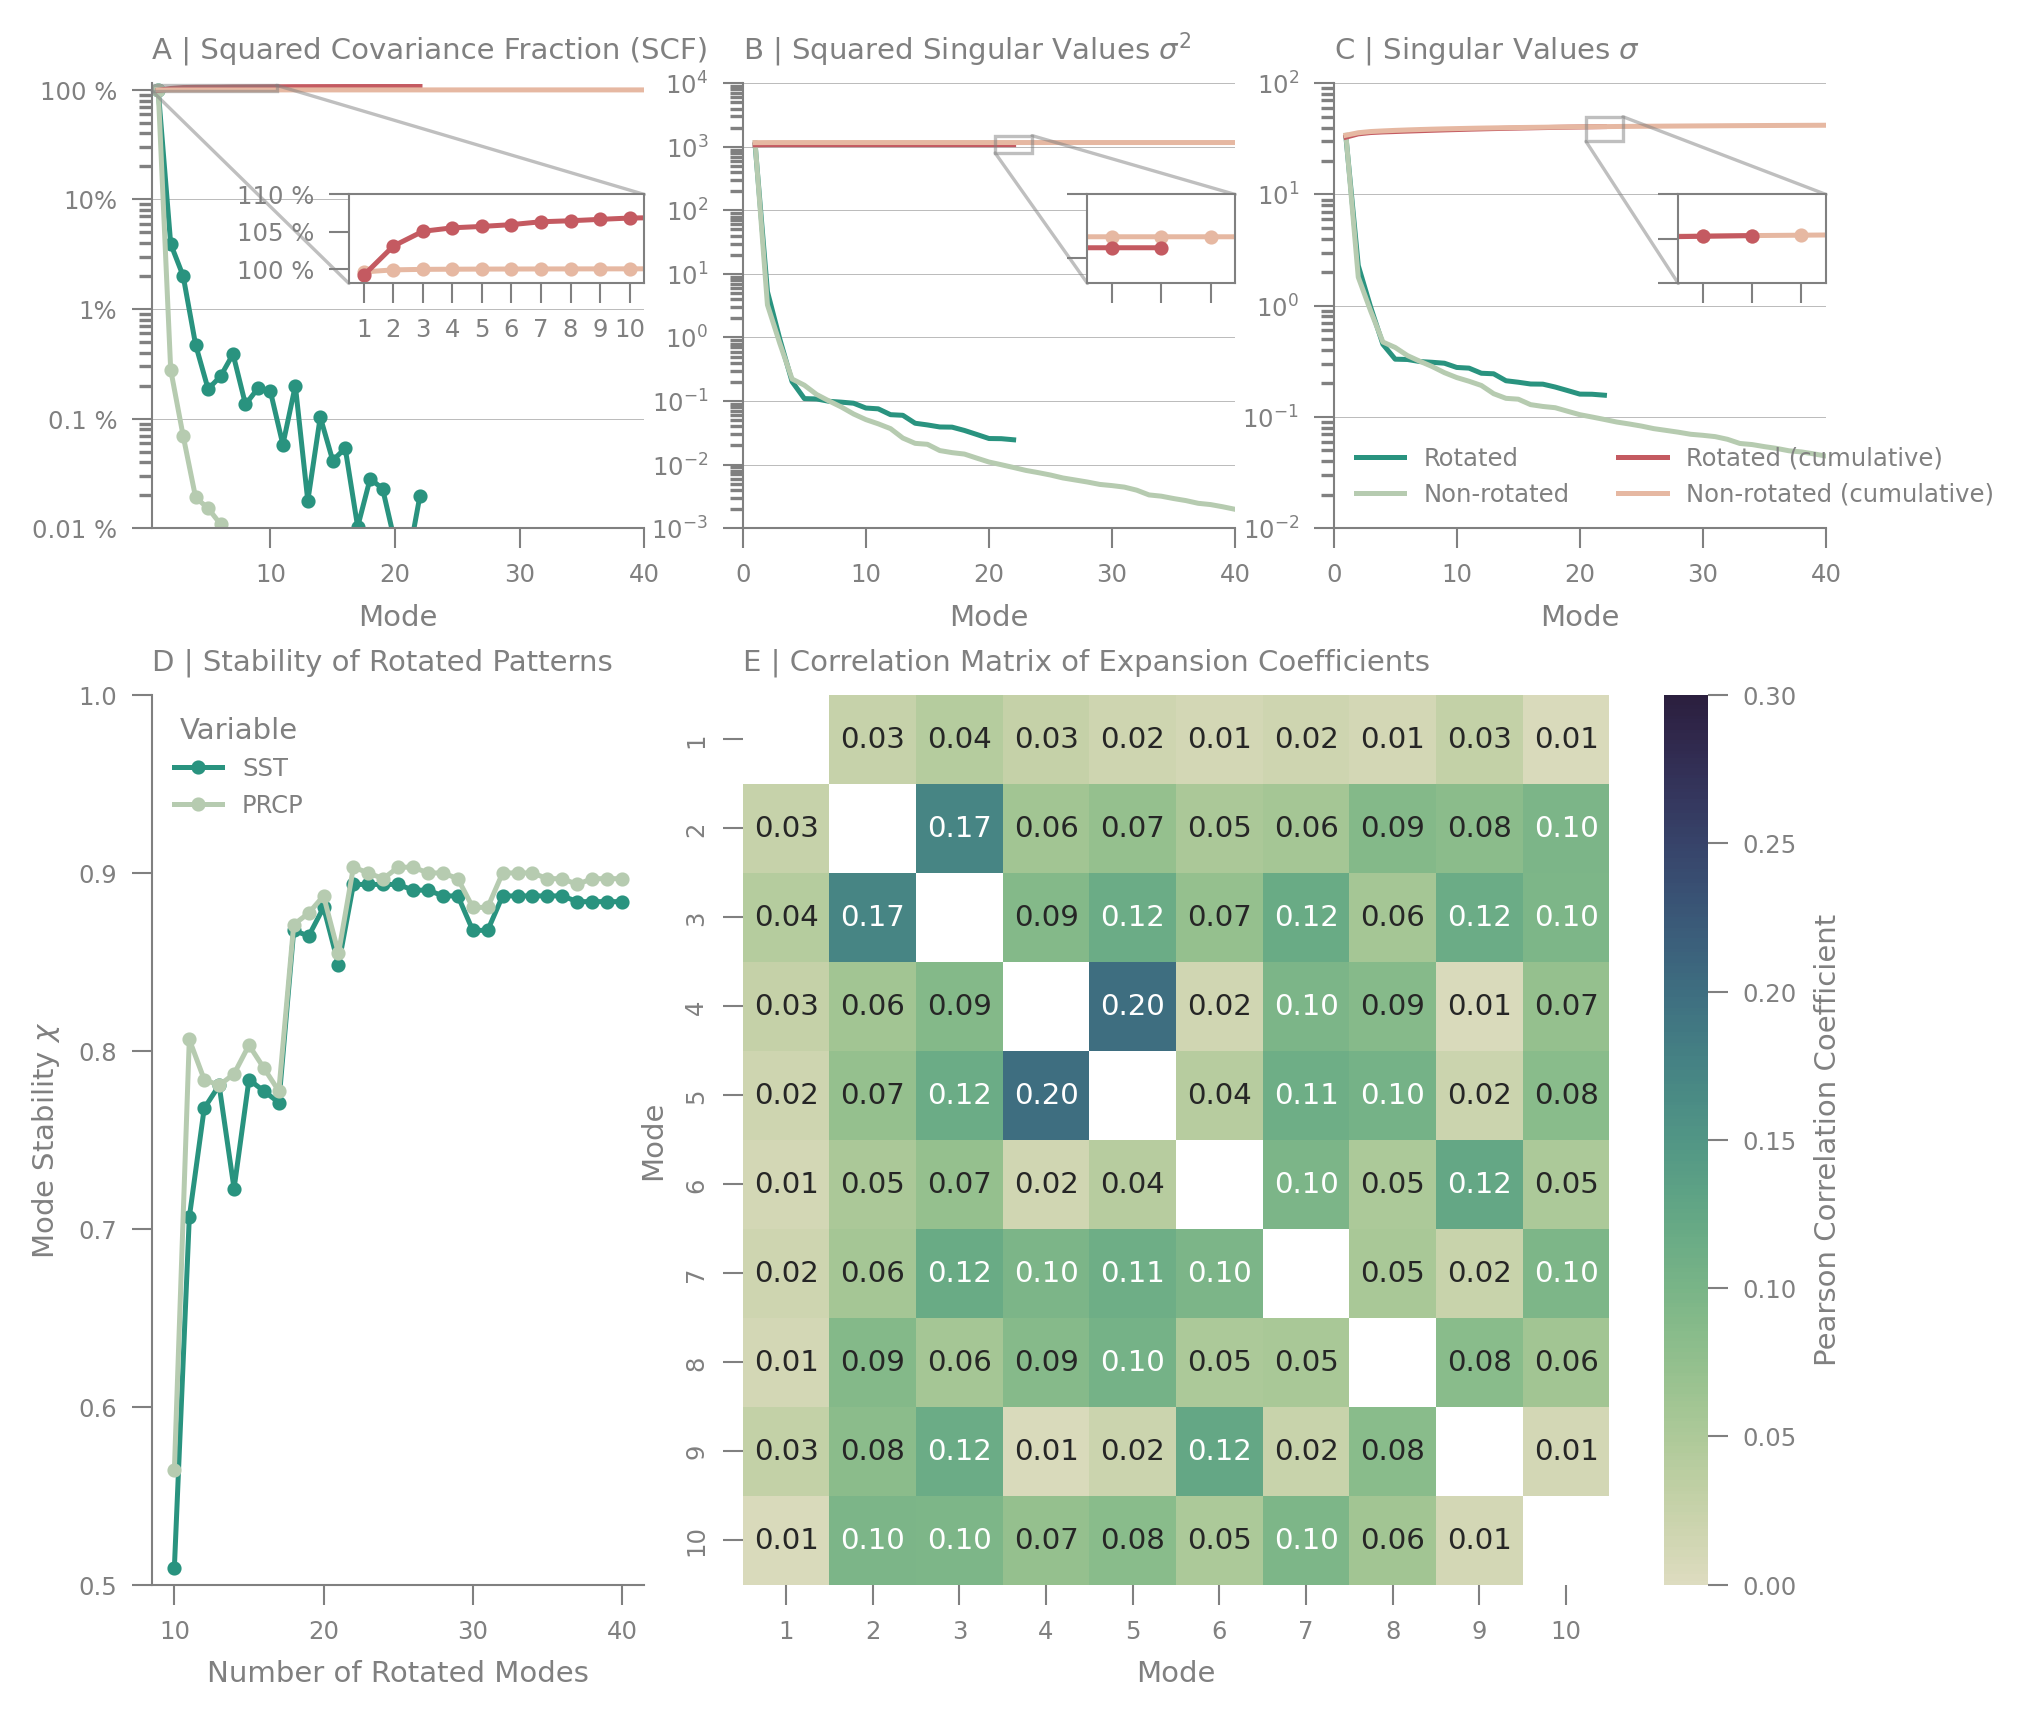
\includegraphics[width=\textwidth]{tele_singular_spectrum}
    \caption[Evaluation of varimax-rotated Hilbert MCA applied to SST and continental precipitation.]{\textbf{Evaluation of varimax-rotated Hilbert MCA applied to SST and precipitation.} \textbf{(A)} Squared covariance fraction (SCF) of the rotated modes, indicating that the SCF does not sum to \qty{100}{\percent} after rotation. The SCF is computed according to Equation~\eqref{eq:theory:mca_scf_residual}. \textbf{(B)} Squared covariance before and after rotation; the inset highlights that squared covariance is not conserved under rotation. Squared covariance is computed according to Equations~\eqref{eq:theory:mca_covariance} (before rotation) and \eqref{eq:theory:mca_covariance_rotated_expansion_coefficients} (after rotation). \textbf{(C)} Covariance (non-squared) before and after rotation; the inset demonstrates that covariance is preserved under rotation. \textbf{(D)} Mode stability index $\kappa$ showing highest stability when 22 modes are rotated for both SST and continental precipitation (PRCP). \textbf{(E)} Pairwise Pearson correlation coefficients among the varimax-rotated expansion coefficients of SST, illustrating generally low correlations between different modes; the diagonal elements are masked for clarity.}
    \label{fig:tele:singular_spectrum}
\end{figure}




\paragraph{Climate Oscillations Indices}
For comparative purposes, we obtained climate indices of monthly means from the Physical Sciences Laboratory (PSL) of the National Oceanic and Atmospheric Administration (NOAA; \url{https://psl.noaa.gov/data/timeseries/month/}), including the Oceanic Niño Index (ONI) provided by the NOAA Climate Prediction Center, the PDO as defined by \citet{mantua_pacific-decadal_2002}, the Indian Ocean Dipole (IOD) as defined by \citet{saji_possible_2003}, and the Atlantic Meridional Mode (AMM) as defined by \citet{chiang_analogous_2004}. We calculated the ENSO Modoki Index (EMI) following \citet{ashok_nino_2007} using the formula $EMI = R_A - \frac{1}{2}R_B - \frac{1}{2}R_C$, where $R$ denotes the area-averaged ERA5 SST anomalies over regions A (\ang{165}E-\ang{140}W; \ang{10}S-\ang{10}N), B (\ang{110}W-\ang{70}W; \ang{15}S-\ang{5}N), and C (\ang{125}E-\ang{145}E; \ang{10}S-\ang{20}N). Additionally, we define an Oceanic Warming Index (OWI) as the area average of ERA5 SST anomalies between \ang{60}S and \ang{70}N, using the same latitude weighting as in our MCA data preparation. 

All indices are smoothed using a centered 7-month moving average to align with our data preprocessing and are restricted to the period from 1940 to 2022. We detrend all indices except the OWI using linear regression to eliminate long-term trends, which could obscure the variability of interest and affect correlation-based analyses. This step was particularly necessary for the IOD, which exhibits a strong trend, but for consistency, we applied the same detrending procedure to all indices. The OWI was excluded from detrending because its trend is deliberate, reflecting large-scale warming. Finally, we centered and standardized all indices to facilitate comparison with the expansion coefficients derived from our MCA.

\paragraph{Power Spectral Density Analysis}
We computed the power spectral density (PSD) for the first 10 expansion coefficients of SST and continental precipitation, along with the climate indices. To ensure consistency, we extracted the real part of the complex-valued expansion coefficients after phase-aligning them. Specifically, for each mode, we adjusted the phase so that the SST heterogeneous pattern reached its maximum absolute value. This alignment was necessary because the singular vectors from our Hilbert MCA are only defined up to an arbitrary phase shift. By standardizing the phase this way, the real part optimally represents lagged variability and captures the dominant temporal signal. 

Before computing the PSD, all time series were linearly detrended. The PSD was then estimated using Welch's Overlapped Segment Averaging (WOSA) method \cite[e.g.,][Section 8.8]{percival_spectral_2020}, with 256 data points per segment, a Hanning window, and \qty{50}{\percent} overlap, yielding six segments in total. All PSDs were normalized to represent the fractional energy density per frequency band.

Approximate confidence intervals for PSDs are often computed using the $\chi^2$ distribution; however, this approach is valid only for a particular frequency and isn't directly applicable across multiple frequencies or the entire frequency range \cite[cf.][p. 468]{priestley_spectral_1981}. Since we don't know in advance which frequencies are of interest, we employed the circular moving block bootstrap~\cite{politis_circular_1991} to estimate confidence intervals for the PSDs. We generated \num{10000} bootstrap samples by resampling the original time series with replacement, using a block length of 9 years. This choice balances the need for sufficient independent bootstrap samples with the requirement for long enough blocks to resolve the frequencies of interest. Note that this choice limits our ability to resolve periodicities longer than 9 years because we effectively scramble the autocorrelation function beyond this time lag. To preserve the annual cycle, we only considered January as a valid starting point for blocks. We computed the PSD for each bootstrap sample, and the $2.5^{\text{th}}$ and $97.5^{\text{th}}$ percentiles of the bootstrap PSDs are used as the lower and upper bounds of the confidence intervals.

Since climate data often exhibit a "red noise" spectrum\footnote{Red noise refers to a type of stochastic process where variability decreases with increasing frequency, resulting in higher power at lower frequencies. This is commonly observed in climate data due to the persistence of long-term variability.}, we compared the PSDs of the expansion coefficients against a theoretical red noise spectrum \cite[e.g.,][Section 10.3]{wilks_statistical_2019}. We estimated the red noise spectrum using a first-order autoregressive process (AR(1)) and compute the theoretical PSD using the formula given by \citet{gilman_power_1963}. The autoregressive coefficient $\rho$ was estimated from the data as the lag-1 autocorrelation coefficient. We then tested the null hypothesis by comparing the spectral density of the data to that of the AR(1) process using the $F$-statistic at a significance level of $\alpha = 0.01$.

% check out \url{https://kls2177.github.io/Climate-and-Geophysical-Data-Analysis/chapters/Week6/filtering_in_freq3.html}}

\section{Results and Discussion}\label{sec:tele:results}

The rotated modes exhibit a more gradual decline in the cumulative squared covariance fraction (SCF) compared to the unrotated solution (Figure~\ref{fig:tele:singular_spectrum}~A). Each of the first 12 modes accounts for more than \qty{0.1}{\percent} of the total squared covariance. A sharp drop in SCF occurs after the $10^{\text{th}}$ mode, where higher modes contribute significantly less and decay exponentially, suggesting they primarily capture noise. Therefore, our analysis focuses on selected modes within the first 10.

We place particular emphasis on modes previously identified in our earlier work \cite{rieger_lagged_2021}, discussing them in detail, while providing only a brief overview of newly identified modes in this chapter. It is important to note that neither the cumulative SCF nor the sum of squared singular values remains conserved under rotation (Figures~\ref{fig:tele:singular_spectrum}~A,~B). Conservation of singular values occurs only in the specific case of orthogonal varimax rotation (Figure~\ref{fig:tele:singular_spectrum}~C).

\begin{figure}
    \centering
    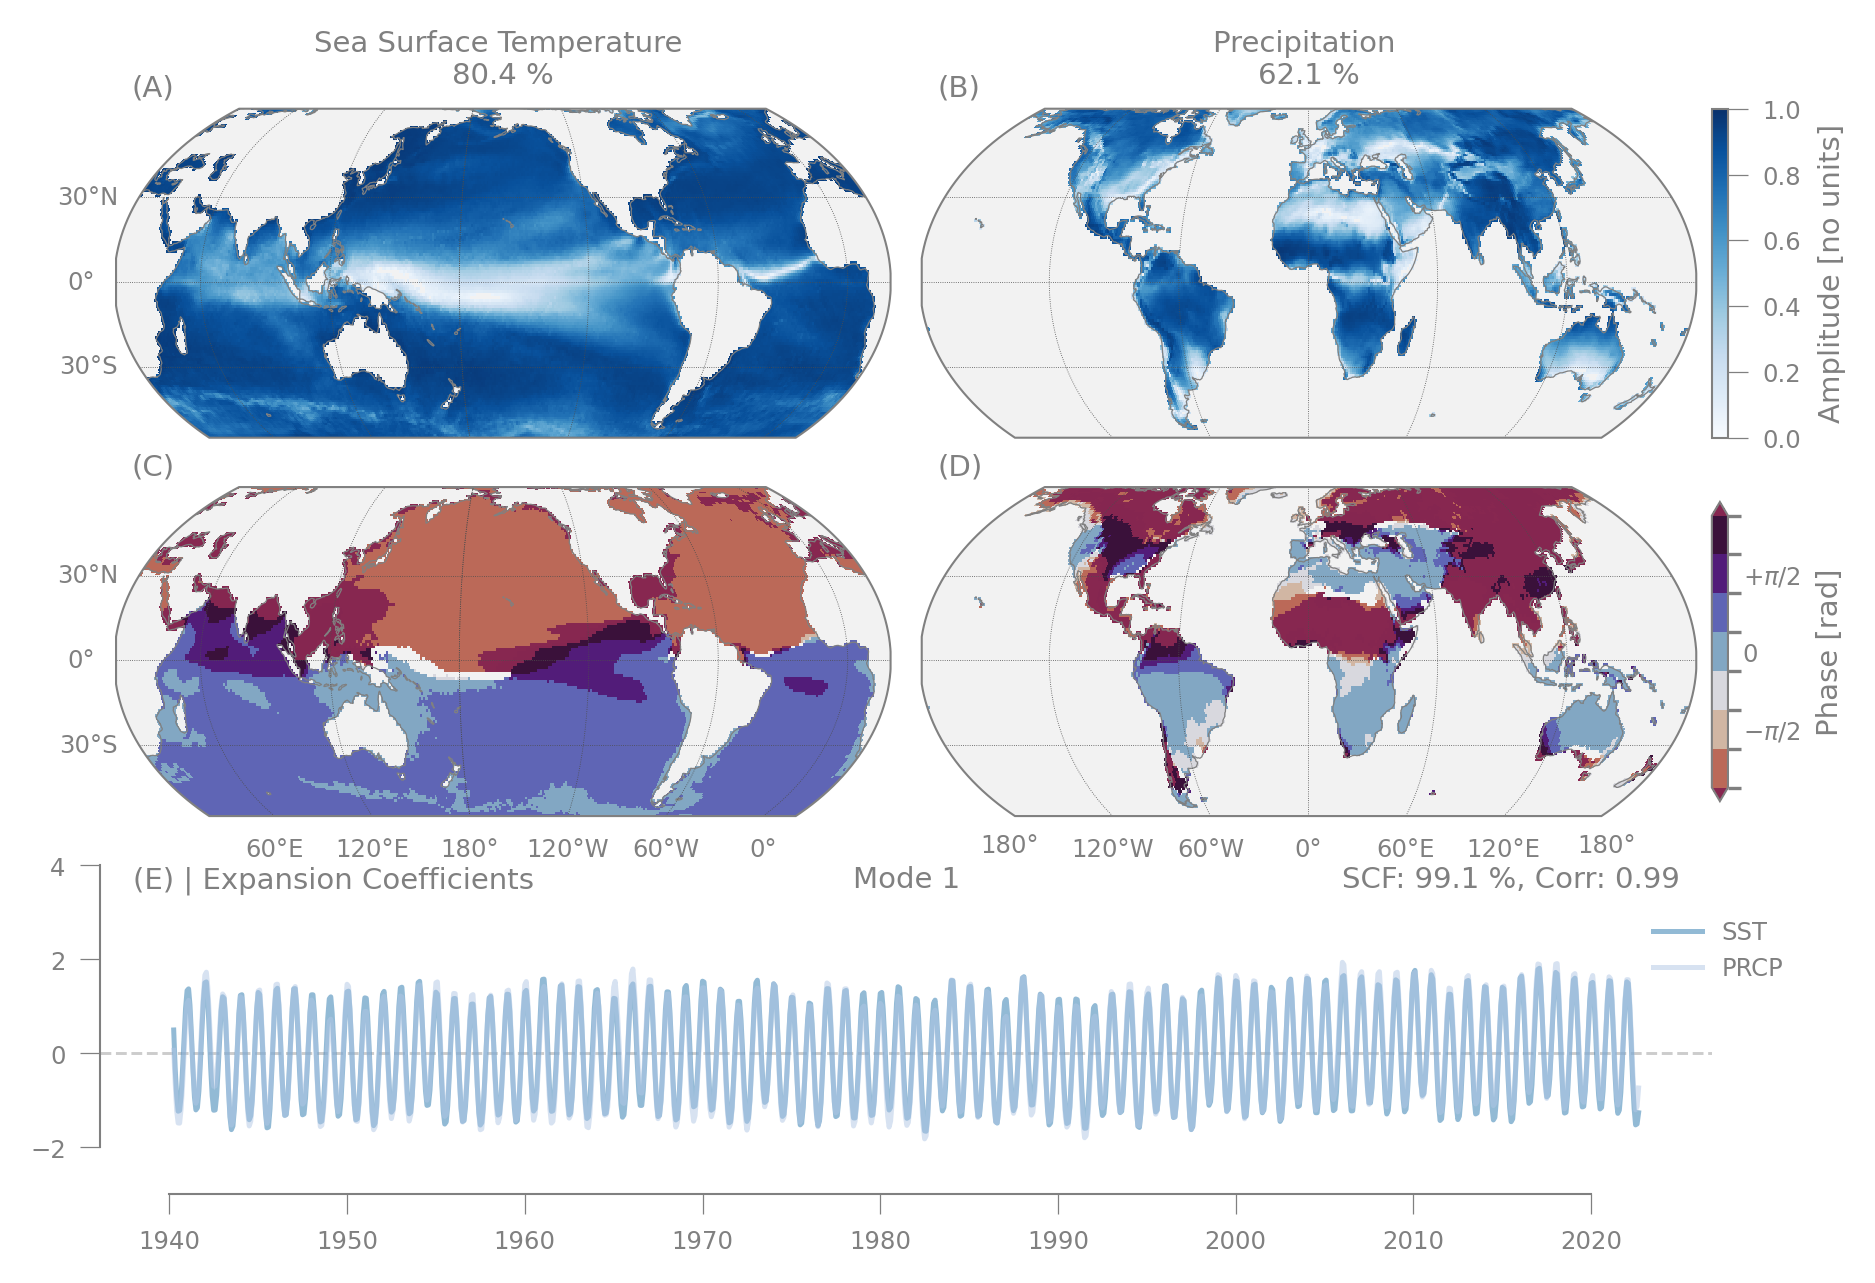
\includegraphics[width=\textwidth]{tele_a100_r22_p1_mode01}
    \caption[Seasonal cycle as represented by mode 1 of varimax-rotated Hilbert MCA applied to SST and continental precipitation.]{\textbf{Seasonal cycle as represented by mode 1 of varimax-rotated Hilbert MCA applied to SST and precipitation.} Absolute values of complex-valued heterogeneous correlation patterns for SST \textbf{(A)} and continental precipitation \textbf{(B)}. Spatial phase patterns for SST \textbf{(C)} and continental precipitation \textbf{(D)}. Associated expansion coefficients \textbf{(E)} for SST (blue) and continental precipitation (light blue). Note that due to the high similarity between the expansion coefficients, their differences are difficult to discern visually. The squared covariance fraction (SCF) indicates the mode's relative importance in summarizing the overall covariability between SST and precipitation. The Pearson correlation coefficient (CORR) between the expansion coefficients reflects the strength of their linkage, while the explained variance for each dataset (noted below the variable name) shows the mode's significance within each dataset. Amplitude and spatial phase are plotted only where p-values, adjusted via the Benjamini-Hochberg correction for multiple testing, are below \num{0.05}. Additionally, the spatial phase is masked in regions where the spatially max-normalized amplitude is below \num{0.125} to eliminate noisy phase values and enhance visualization. For clarity, the spatial phase is discretized into bins of 45 degrees ($\pi/4$ radians).}
    \label{fig:tele:mode01_a100}
\end{figure}



\begin{table}[th]
    \caption[Summary of the first ten rotated modes of varimax-rotated Hilbert MCA applied to SST and continental precipitation.]{\textbf{Summary of the first ten rotated modes of varimax-rotated Hilbert MCA applied to SST and continental precipitation.} The table presents key statistical properties of the first ten modes obtained from the analysis. Listed are the squared covariance fraction (SCF) $f_k$ of each mode $k$, the absolute Pearson correlation coefficient between the expansion coefficients of SST and precipitation, $\rho_k$, and the explained variance for SST and precipitation, $f_k^{\text{SST}}$ and $f_k^{\text{PRCP}}$, respectively. If applicable, the associated climate index, $i$, is also indicated along with the Pearson correlation coefficient between the real part of the expansion coefficient of SST and the climate index, $\rho_k^i$.}
    \centering
    \label{tab:tele:summary}
    \hspace*{-.2cm} 
    \makebox[\textwidth][c]{
        \begin{tabular}{ccccc@{\hskip 50pt}cc}
            \toprule
            \textsc{Mode} $k$ & $f_k$ [\unit{\percent}] & $\rho_k$ & $f_k^{\text{SST}}$ [\unit{\percent}] & $f_k^{\text{PRCP}}$ [\unit{\percent}] & \textsc{Climate Index} $i$ & $\rho_k^i$ \\
            \midrule
            1 & 99.1 & 0.99 & 80.4 & 62.1 & - & - \\
            2 & 3.9 & 0.91 & 5.8 & 4.6 & ONI & 0.92 \\
            3 & 2.0 & 0.80 & 3.0 & 1.4 & OWI & 0.78 \\
            4 & 0.5 & 0.82 & 1.1 & 1.0 & EMI & 0.56 \\
            5 & 0.4 & 0.82 & 0.8 & 0.7 & - & - \\
            6 & 0.2 & 0.85 & 0.7 & 0.8 & AMM & 0.75 \\
            7 & 0.2 & 0.79 & 0.6 & 0.6 & - & - \\
            8 & 0.2 & 0.84 & 0.9 & 0.6 & - & - \\
            9 & 0.2 & 0.78 & 0.9 & 0.8 & PDO & 0.59 \\
            10 & 0.2 & 0.83 & 0.4 & 1.2 & IOD & 0.49 \\
            \bottomrule
        \end{tabular}
    }
\end{table}

\paragraph{Mode 1---The Seasonal Cycle} 
Mode 1 accounts for more than \qty{99}{\percent} of the squared covariance between SST and continental precipitation (Table~\ref{tab:tele:summary}) and exhibits a clear one-year periodicity, unequivocally representing the annual cycle (Figures~\ref{fig:tele:mode01_a100}, \ref{fig:tele:psd}~A). This mode shows a very strong link between SST and precipitation, evidenced by a Pearson correlation coefficient of $r_{ec,1}=0.99$ between their expansion coefficients. As expected, the annual cycle manifests globally in both variables, with strong expressions in the extratropics for SST and within the tropics for precipitation. Exceptions to this pattern occur in transition zones, such as north of the Arabian Sea, where precipitation shifts between summer and winter-dominated regimes over a narrow region, or in areas with multiple rainy seasons like central East Africa.

The phase functions (Figures~\ref{fig:tele:mode01_a100}~C, D) correctly separate the seasonal cycle according to the timing of the annual peak, identifying, for example, the anticorrelation (phase shift of approximately $\pi$) between the northern and southern oceans. In SST, we observe that the eastern equatorial Pacific and the equatorial Indian Ocean exhibit a positive phase shift of $+\pi/4$ (about six weeks) relative to the dominant oceanic seasonal cycle. On the continents, the phase function illustrates the division between January-February (light blue) and July-August (dark red) dominated rainfall systems, identifying corresponding transition zones such as over the South American rainforest and central North America. It also highlights interesting dynamical regions that stand out from their surroundings, namely the west and east coasts of North America, the Mediterranean region, and, to a lesser extent, the East Asian monsoon region in China.

We also note that this first mode explains significantly more variance in SST (\qty{80.4}{\percent}) than in continental precipitation (\qty{62.1}{\percent}). This is expected because the seasonal cycle is a more dominant feature in SST, whereas precipitation is generally a noisier variable with a more complex spatiotemporal structure. Specifically, precipitation is more directly influenced by atmospheric variability, which exhibits high internal variability. Additionally, the ocean's thermal inertia allows it to absorb or release large amounts of heat with only minor temperature changes, making SSTs generally less variable than atmospheric variables. Finally, while SSTs change smoothly and slowly over vast spatial scales, continental precipitation is highly localized, so interannual variations in global circulation patterns can produce drastic changes in local precipitation patterns.

\begin{figure}
    \centering
    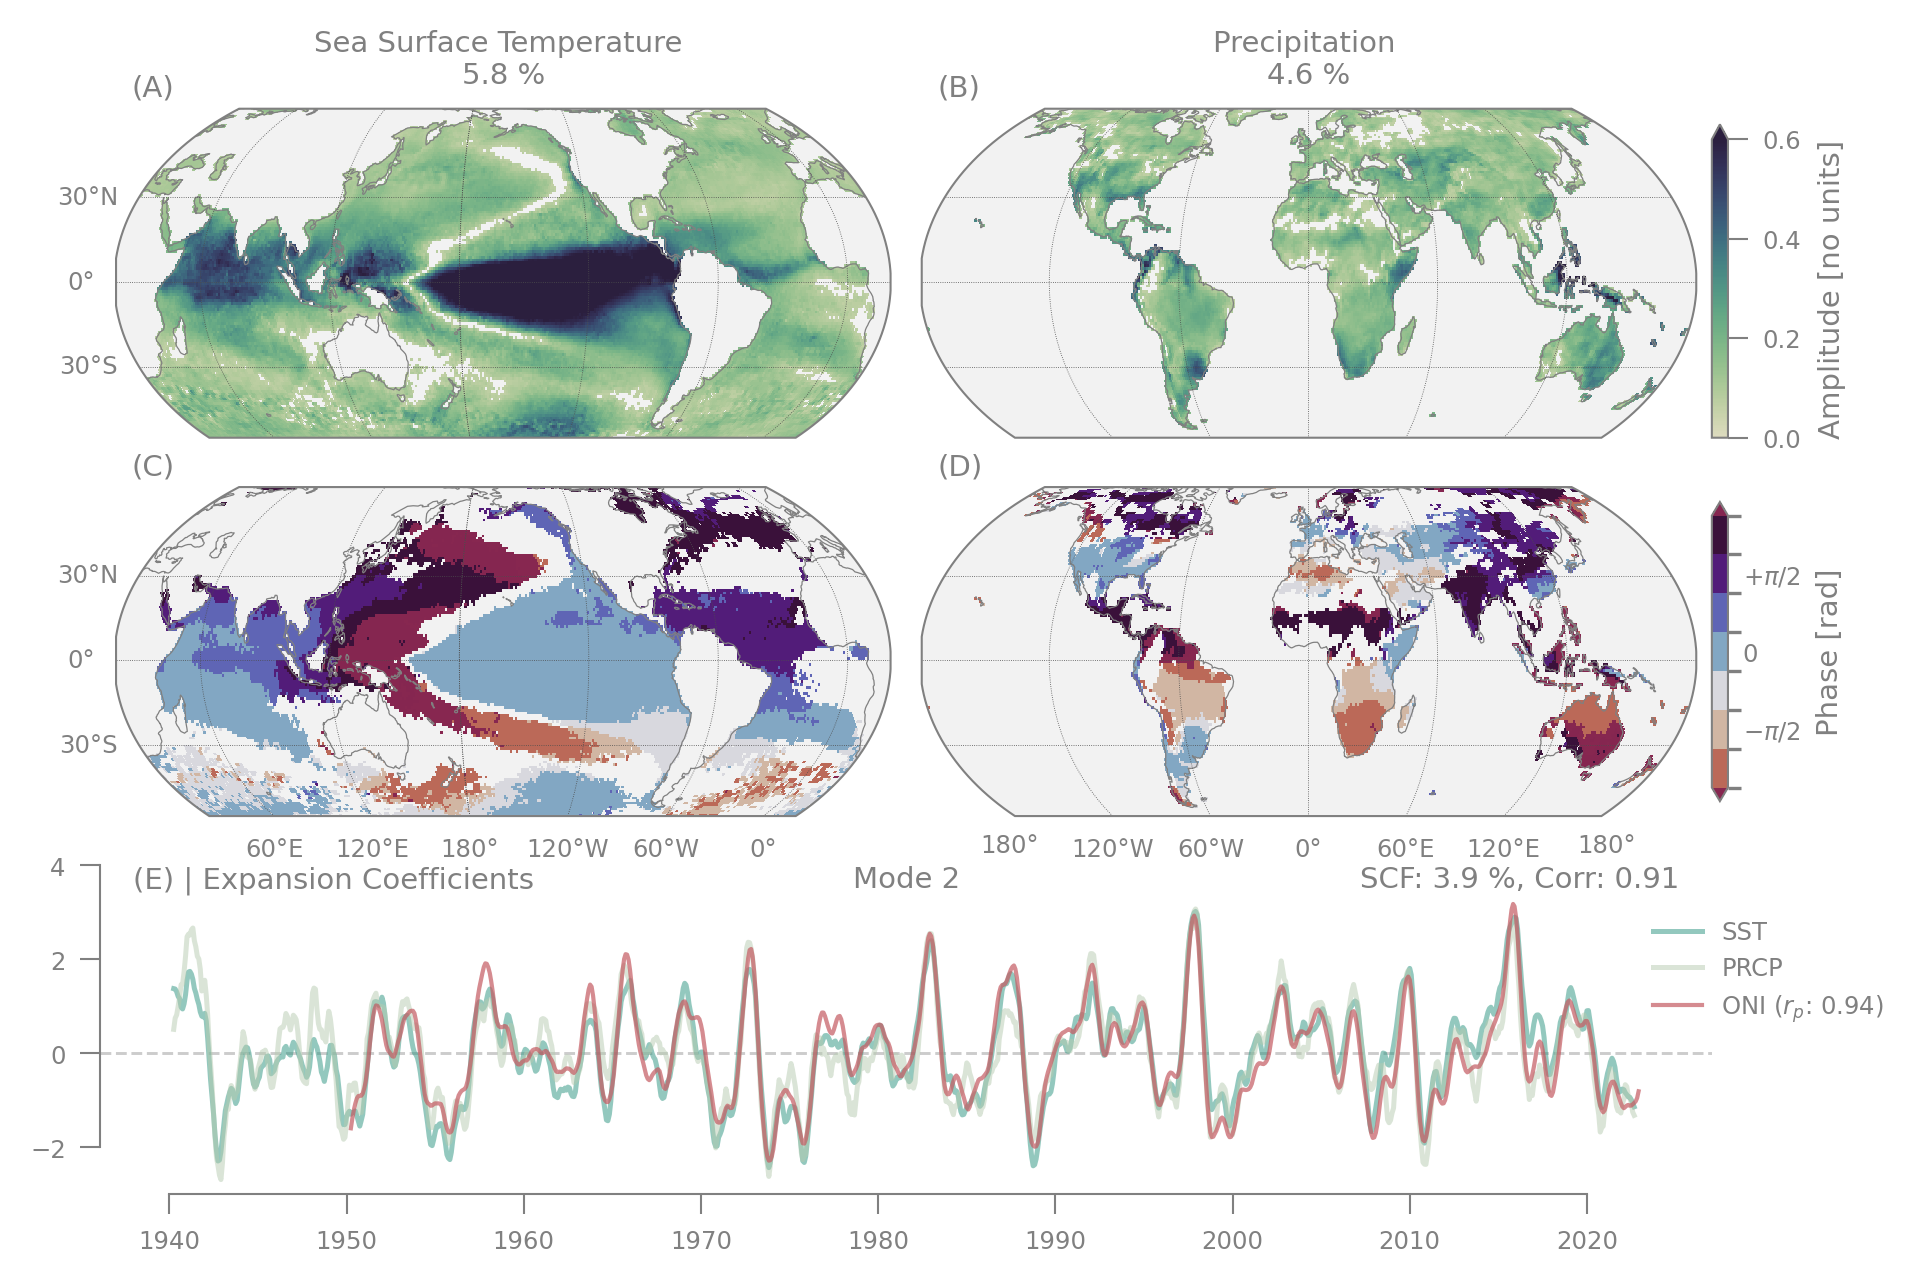
\includegraphics[width=\textwidth]{tele_a100_r22_p1_mode02}
    \caption[ENSO as represented by mode 2 of varimax-rotated Hilbert MCA applied to SST and continental precipitation.]{\textbf{ENSO as represented by mode 2 of varimax-rotated Hilbert MCA applied to SST and continental precipitation.} The orange line represents the Oceanic Niño Index (ONI) for comparison, along with its Pearson correlation coefficient with the SST expansion coefficients. For more details, refer to the description in Figure~\ref{fig:tele:mode01_a100}.}
    \label{fig:tele:mode02_a100}
\end{figure}



\paragraph{Mode 2---ENSO} 
Mode 2 is strongly associated with the ENSO phenomenon, exhibiting a characteristic SST pattern along the tropical Pacific (Figure~\ref{fig:tele:mode02_a100}). This pattern aligns with the dominant interannual variability in SSTs in the tropical Pacific (Figure~\ref{fig:tele:trends}~C). The expansion coefficients of SST for this mode show a high correlation with the ONI, with a Pearson correlation coefficient of $\rho_2^{\text{ONI}}=0.92$ (Table~\ref{tab:tele:summary}), further reinforcing its link to ENSO. Several of the teleconnections identified in Figures~\ref{fig:tele:mode02_a100}~A-B have been previously documented and analyzed. For instance, during El Niño events, increased SSTs in the central and eastern Pacific and lower SSTs in the western Pacific positively correlate with increased rainfall along the west coast and southeastern coast of South America \cite{tedeschi_influences_2013}, the east and west coasts of North America \cite{ropelewski_north_1986}, the East Asian monsoon region \cite{wen_direct_2019}, and the Horn of Africa \cite{indeje_enso_2000}. Simultaneously, precipitation decreases in northern South America \cite{tedeschi_influences_2013}, Oceania \cite{dai_global_2000}, South Africa \cite{gaughan_inter-_2016}, and the Indian monsoon region \cite{cherchi_influence_2013}. During La Niña events, these correlations are reversed. More recently, similar teleconnections have been identified using event coincidence analysis \cite{wiedermann_differential_2021}. For a relatively recent summary of established ENSO-related rainfall patterns during El Niño and La Niña, see \citet{lenssen_seasonal_2020}.

Furthermore, our results demonstrate the lagged dynamics between the core ENSO region in the western and central Pacific and other regions such as the Indian Ocean \cite{krishnamurthy_variability_2003}, the South China Sea \cite{klein_remote_1999}, and the tropical North Atlantic \cite{enfield_tropical_1997, saravanan_interaction_2000, alexander_influence_2002, chiang_tropical_2002}, consistent with previous studies. ENSO-related SST teleconnections in remote oceans often occur with delays: the Indian Ocean typically peaks 3 months, and the South China Sea and tropical North Atlantic about 5 months after the SST peak in the Pacific ENSO region \cite{enfield_tropical_1997, klein_remote_1999, saravanan_interaction_2000}. The mechanism behind these lagged responses involves characteristic atmospheric circulation changes during El Niño events, leading to alterations in cloud cover and evaporation over remote oceans, resulting in increased net heat flux and SSTs \cite{lau_role_1996, klein_remote_1999}.



\begin{center}
    
\includegraphics[width=\textwidth]{tele_psd}
    \medskip
    \emph{(Caption on next page.)}
    % a little hack to add the caption to the next page; the figure number in the LOF needs to be manually adjusted
    \addcontentsline{lof}{figure}{7.4\quad Power spectral densities (PSDs) of the first 10 expansion coefficients.}
\end{center}

\begin{figure}
    \centering
    \caption[Power spectral densities (PSDs) of the first 10 expansion coefficients.]{\textbf{Power spectral densities (PSDs) of the first 10 expansion coefficients.} Normalized PSDs of the real part of the expansion coefficients for the first 10 modes of SST and continental precipitation.  When appropriate, the PSDs of corresponding climate indices were added: Oceanic Niño Index (ONI), the Pacific Decadal Oscillation (PDO), the Atlantic Meridional Mode (AMM), the ENSO Modoki Index (EMI), and the Indian Ocean Dipole (IOD). The PSDs are normalized to represent the fraction of energy density per frequency band. The shaded areas represent the \qty{95}{\percent} confidence intervals estimated using the circular moving block bootstrap. The solid red line indicates the theoretical `red noise' spectrum, and the dashed red lines show the $F$-statistic for the null hypothesis that the data PSD is equal to the AR(1) process PSD.}
    \label{fig:tele:psd}
\end{figure}

However, due to the broadband frequency spectrum of the SST expansion coefficients (Figure~\ref{fig:tele:psd}~B), with most energy between periodicities of roughly 2 and 5 years, the phase cannot be directly translated into a precise time shift. Assuming these periodicity limits, we can compute an approximate time shift. For example, the tropical Atlantic exhibits a phase shift of $+\pi/2$, translating into time shifts bounded between 6 and 15 months, which is close to but slightly larger than the observed average time lag of 5 months. Nevertheless, the tropical North Atlantic clearly shows more positive phase values compared to the Pacific El Niño region, indicating it is positively time-shifted relative to the Pacific.

Recently, \citet{scaife_enso_2024} provided evidence for an even longer time lag—a one-year lagged extratropical response to ENSO—most pronounced in the North Atlantic. While they used sea surface pressure as the observational variable to assess the ENSO teleconnection, our SST-based analysis also indicates a weak signal of shared variability with ENSO in the North Atlantic, with a phase shift of approximately $+3\pi/4$. Using the periodicity limits from our analysis, this lag corresponds to time shifts between 9 and 22.5 months, aligning well with the reported one-year lagged response by \citet{scaife_enso_2024}.

Considering all the lagged covariance collectively, ENSO accounts for approximately \qty{5.8}{\percent} of SST variability and about \qty{4.6}{\percent} of continental precipitation variability since 1940.


\begin{figure}
    \centering
    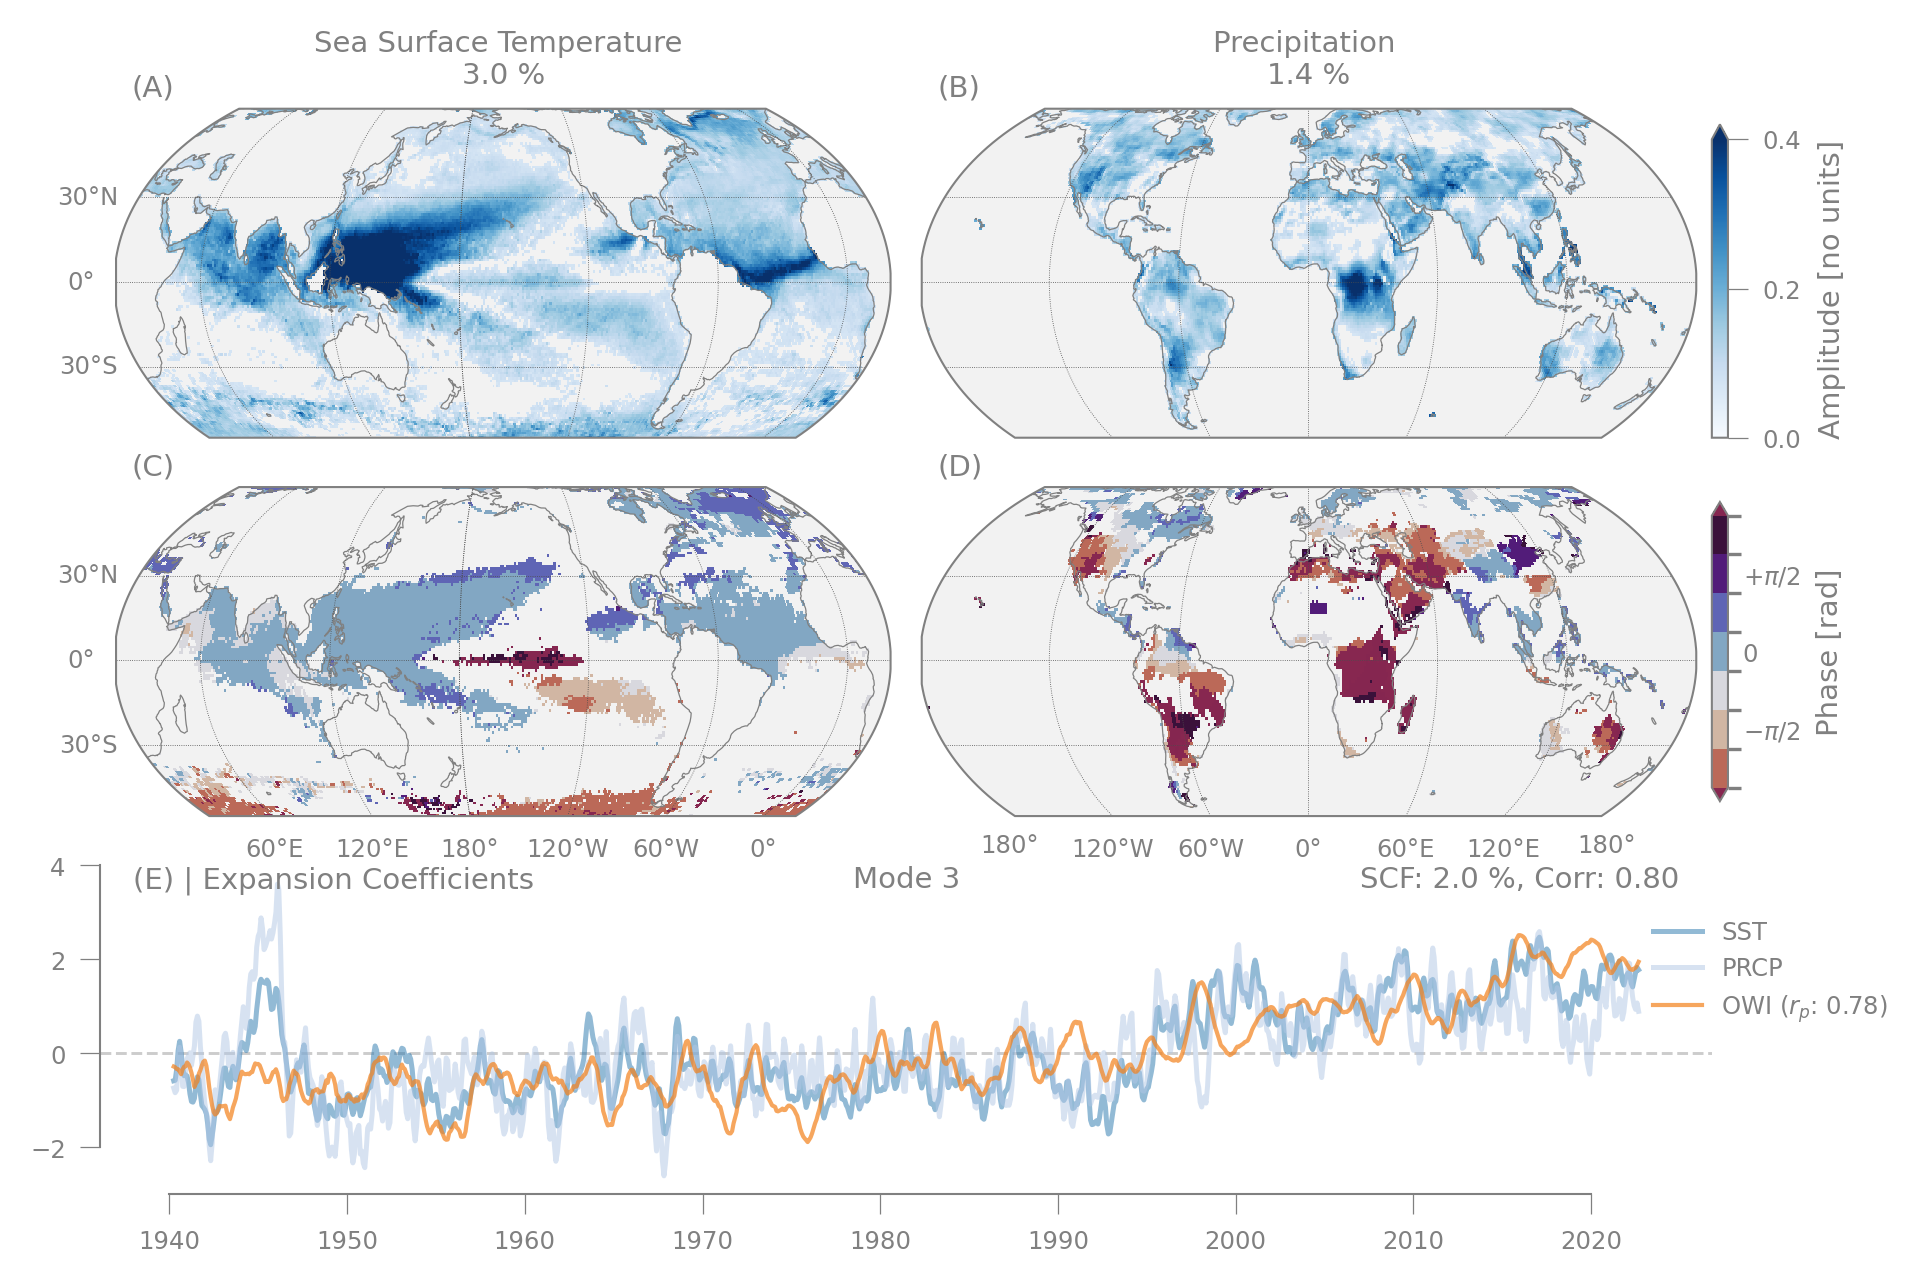
\includegraphics[width=\textwidth]{tele_a100_r22_p1_mode03}
    \caption[Tropical long-term trends as represented by mode 3 of varimax-rotated Hilbert MCA applied to SST and continental precipitation.]{\textbf{Tropical long-term trends as represented by mode 3 of varimax-rotated Hilbert MCA applied to SST and continental precipitation.} The orange line represents the Oceanic Warming Index (OWI) for comparison, along with its Pearson correlation coefficient with the SST expansion coefficients. For more details, refer to the description in Figure~\ref{fig:tele:mode01_a100}.}
    \label{fig:tele:mode03_a100}
\end{figure}



\begin{figure}
    \centering
    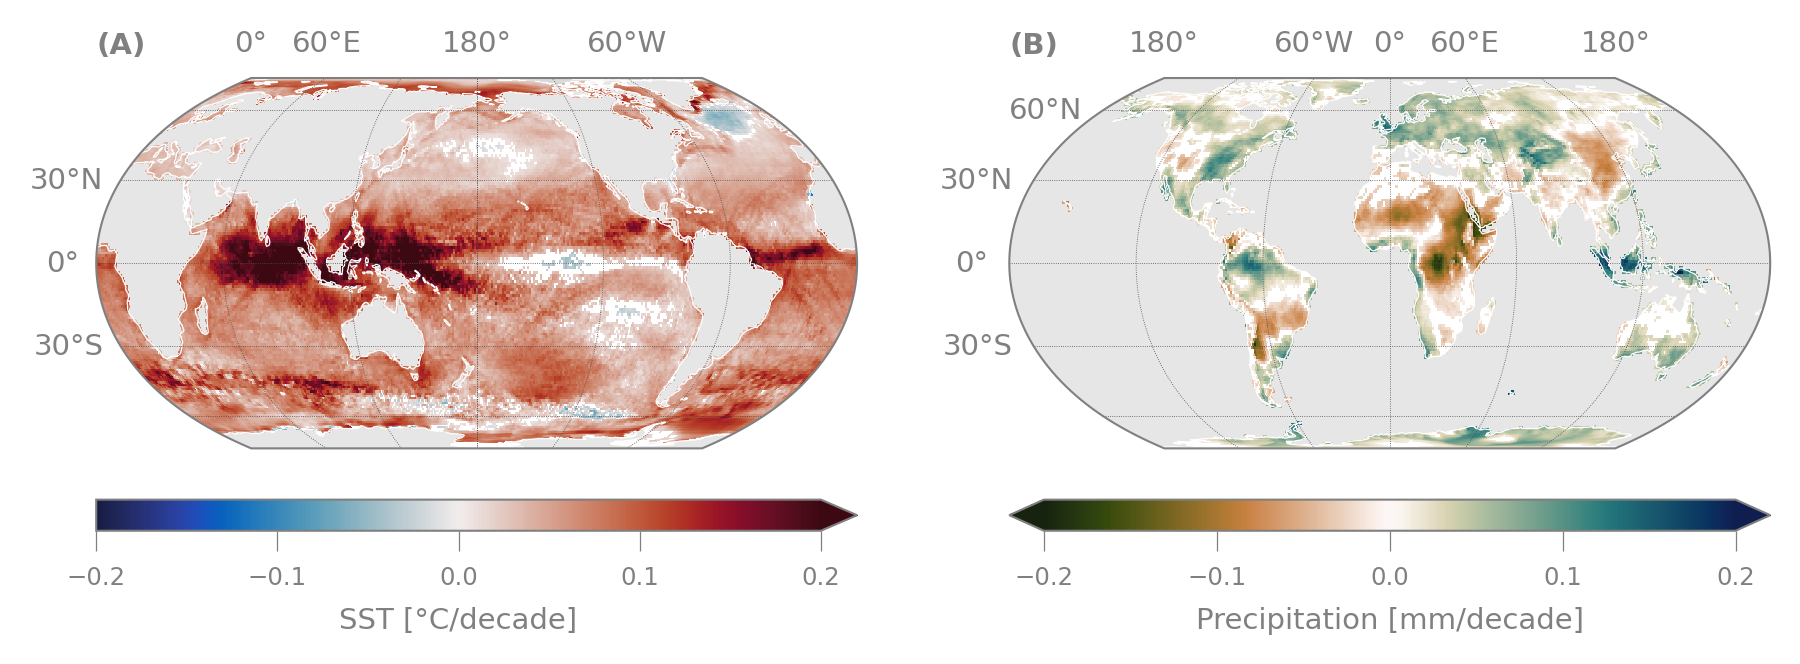
\includegraphics[width=\textwidth]{tele_trends}
    \caption[Key characteristics of sea surface temperature (SST) and continental precipitation from ERA5 data.]{\textbf{Key characteristics of sea surface temperature (SST) and continental precipitation from ERA5 data.} The first column \textbf{(A, C, E)} presents SST, while the second column \textbf{(B, D, F)} shows continental precipitation. The mean state \textbf{(A, B)} represents the average of annual means over the reference period 1991-2020, with SST in degrees Celsius (\unit{\degreeCelsius}) and total annual precipitation in millimeter (\unit{mm}). Annual variability \textbf{(C, D)} is quantified as the standard deviation of annual means within the same reference period, reflecting interannual fluctuations after averaging out the seasonal cycle. Linear trends of annual means from 1940 to 2022 per decade (dc) \textbf{(E, F)} are shown only in regions where the adjusted $p$-value, corrected for multiple testing using the Benjamini-Hochberg method \cite{benjamini_controlling_1995}, is less than $0.05$. SST trends indicate near-global warming, except for a cooling region in the northwestern Atlantic, known as the "cold blob" \cite{drijfhout_is_2012,rahmstorf_exceptional_2015,li_century-long_2022}. Precipitation trends exhibit strong regional variations, with the most pronounced changes occurring in the tropics and subtropics. The trends are largely in agreement with observational datasets \cite{ipcc_water_2023, ipcc_ocean_2023}.}
    \label{fig:tele:trends}
\end{figure}



\paragraph{Mode 3---Tropical Warming Trend} 
Mode 3 captures long-term variability in SST and precipitation, characterized by a slow but accelerating positive trend. Spatially, warming patterns appear across all major ocean basins, with a distinct focus along the equator. The SST spatial amplitude functions suggest a stronger warming effect in the northwestern tropics and a weaker response in the southeastern tropics (Figure~\ref{fig:tele:mode03_a100}~A). Precipitation patterns exhibit a similarly widespread distribution, with the strongest correlations centered over tropical Africa (Figure~\ref{fig:tele:mode03_a100}~B). Other regions with notable but lower correlations include Oceania, South and North America, and Central Asia.

Examining the phase functions, SSTs are increasing across nearly all high-amplitude regions (phase shift near zero), except for the Southern Ocean around \ang{60} S, where the phase function (close to $\pm \pi$) suggests a decrease, albeit with low spatial correlation. A similar pattern emerges in precipitation trends, with central Africa experiencing a decrease, while Oceania, for example, shows an increase. Due to the broadband power spectrum of the expansion coefficients (Figure~\ref{fig:tele:psd}~C), phase values can only be meaningfully interpreted at $0$ (correlation) and $\pm \pi$ (anticorrelation). Intermediate phase shifts, such as $-\pi/4$ in western Australia, lack a straightforward interpretation. 

The long-term trend visible in the expansion coefficients suggests a connection to global warming. A strong correlation with the OWI, $\rho_3^{\text{OWI}}=0.78$, supports this idea (Figure~\ref{fig:tele:mode03_a100}~E). Additionally, the slightly stronger SST warming in the Northern Hemisphere aligns with the asymmetric response of the trade winds to global warming \cite{xie_global_2010}, and the pronounced warming in the western Pacific and Atlantic basins is consistent with enhanced ocean heat transport \cite{xie_global_2010, hannachi_archetypal_2017}. However, the spatial patterns of Mode 3 diverge from those typically associated with global warming. Linear SST trends from 1940-2022 (computed from ERA5 data) show a more uniform warming pattern across the oceans (Figure~\ref{fig:tele:trends}~E), with a few exceptions, such as the "cold blob" in the northwestern Atlantic \cite{drijfhout_is_2012,rahmstorf_exceptional_2015,li_century-long_2022}. In contrast, mode 3 highlights a dominant equatorial warming pattern, whereas linear trends suggest that warming is stronger at higher latitudes than at the equator. While the regional patterns of precipitation trends in mode 3 align well with the linear precipitation trends derived directly from ERA5 (Figure~\ref{fig:tele:trends}~F), the SST patterns show notable differences.

One possible reason for this discrepancy lies in biases in the ERA5 dataset, particularly in regions and time periods with sparse observational coverage \cite{soci_era5_2024}, such as central Africa and pre-satellite-era records. These biases are known to influence precipitation estimates \cite{lavers_evaluation_2022}, yet they should not affect the consistency between the linear trends and MCA-based spatial patterns, as both are derived from the same dataset. While ERA5 might underestimate the severity of the central African drying trend compared to observational datasets \cite{contractor_changes_2021, ipcc_water_2023}, this alone does not explain why the SST patterns in mode 3 differ so strongly from linear trends. Precipitation trends largely align with existing observational data \cite{ipcc_water_2023}, whereas SST patterns show a pronounced deviation \cite{ipcc_ocean_2023}.

A more plausible explanation is that SST warming did not occur simultaneously across the globe. Different regions warmed at different times due to regional climate dynamics, ocean currents, and atmospheric interactions. The North Atlantic and Arctic warmed earlier due to Arctic amplification and sea ice loss \cite{tokinaga_early_2017,hegerl_early_2018}, while the eastern Pacific warmed more slowly due to strong upwelling of cold deep water and natural variability \cite{heede_eastern_2021}. The Southern Ocean, similarly, experienced delayed warming due to wind-induced mixed layer deepening effectively buffering surface heating \cite{zhang_summer_2024}. Since the Hilbert transformation used in MCA interprets time series in terms of their frequency composition, a long-term warming trend can be conceptualized as the rising edge of a sinusoidal wave. A delayed onset of warming alters the frequency composition rather than inducing a simple phase shift. Because different regions warmed at different times, their associated frequency distributions vary, and MCA may separate these trends into different modes rather than capturing them as a single coherent pattern.

The dominance of tropical SSTs in this mode, rather than Arctic SSTs, where warming rates are higher (Figure~\ref{fig:tele:trends}~E), suggests that precipitation trends may be the primary driver. Tropical and subtropical regions exhibit much greater interannual precipitation variability than extratropical regions (Figure~\ref{fig:tele:trends}~D), and these regions also experience the strongest long-term trends (Figure\ref{fig:tele:trends}~F). Consequently, this mode likely represents precipitation trends that coincide temporally with SST warming trends, rather than directly reflecting global SST trends. The prominence of tropical SSTs is reasonable given the strong causal link between tropical SSTs and tropical precipitation \cite[e.g.][]{mcphaden_enso_2006}.

Another factor to consider is that global warming is inherently nonlinear due to various feedback mechanisms \cite{bony_how_2006,roe_why_2007}. Arctic amplification, for instance, leads to significantly faster warming in the Arctic compared to the global average due to factors such as the ice-albedo effect, increased water vapor, and changes in circulation patterns \cite{serreze_processes_2011,previdi_arctic_2021}. This is evident in the stronger warming trends at \ang{60}~N (Figure~\ref{fig:tele:trends}~E). If polar regions not only warm at a proportionally higher rate than the tropics but also exhibit an accelerating warming rate over time (which seems to be the case \cite{chen_assessments_2019}), MCA's linear decomposition may fail to capture this complexity. As a result, the warming pattern may be split into multiple modes rather than appearing as a single unified signal.

Ultimately, the spatial patterns of mode 3 likely reflect a combination of these effects. The observed discrepancy in SST trends arises because MCA isolates dominant co-variability patterns rather than directly capturing linear trends. This mode is best interpreted as a tropical precipitation-driven pattern that coincides with SST warming trends, rather than a direct representation of global SST trends. Additionally, the mode's separation from high-latitude warming signals is likely a result of both the regional timing of warming onset and the limitations of MCA's linear framework in representing nonlinear climate processes.


\begin{figure}
    \centering
    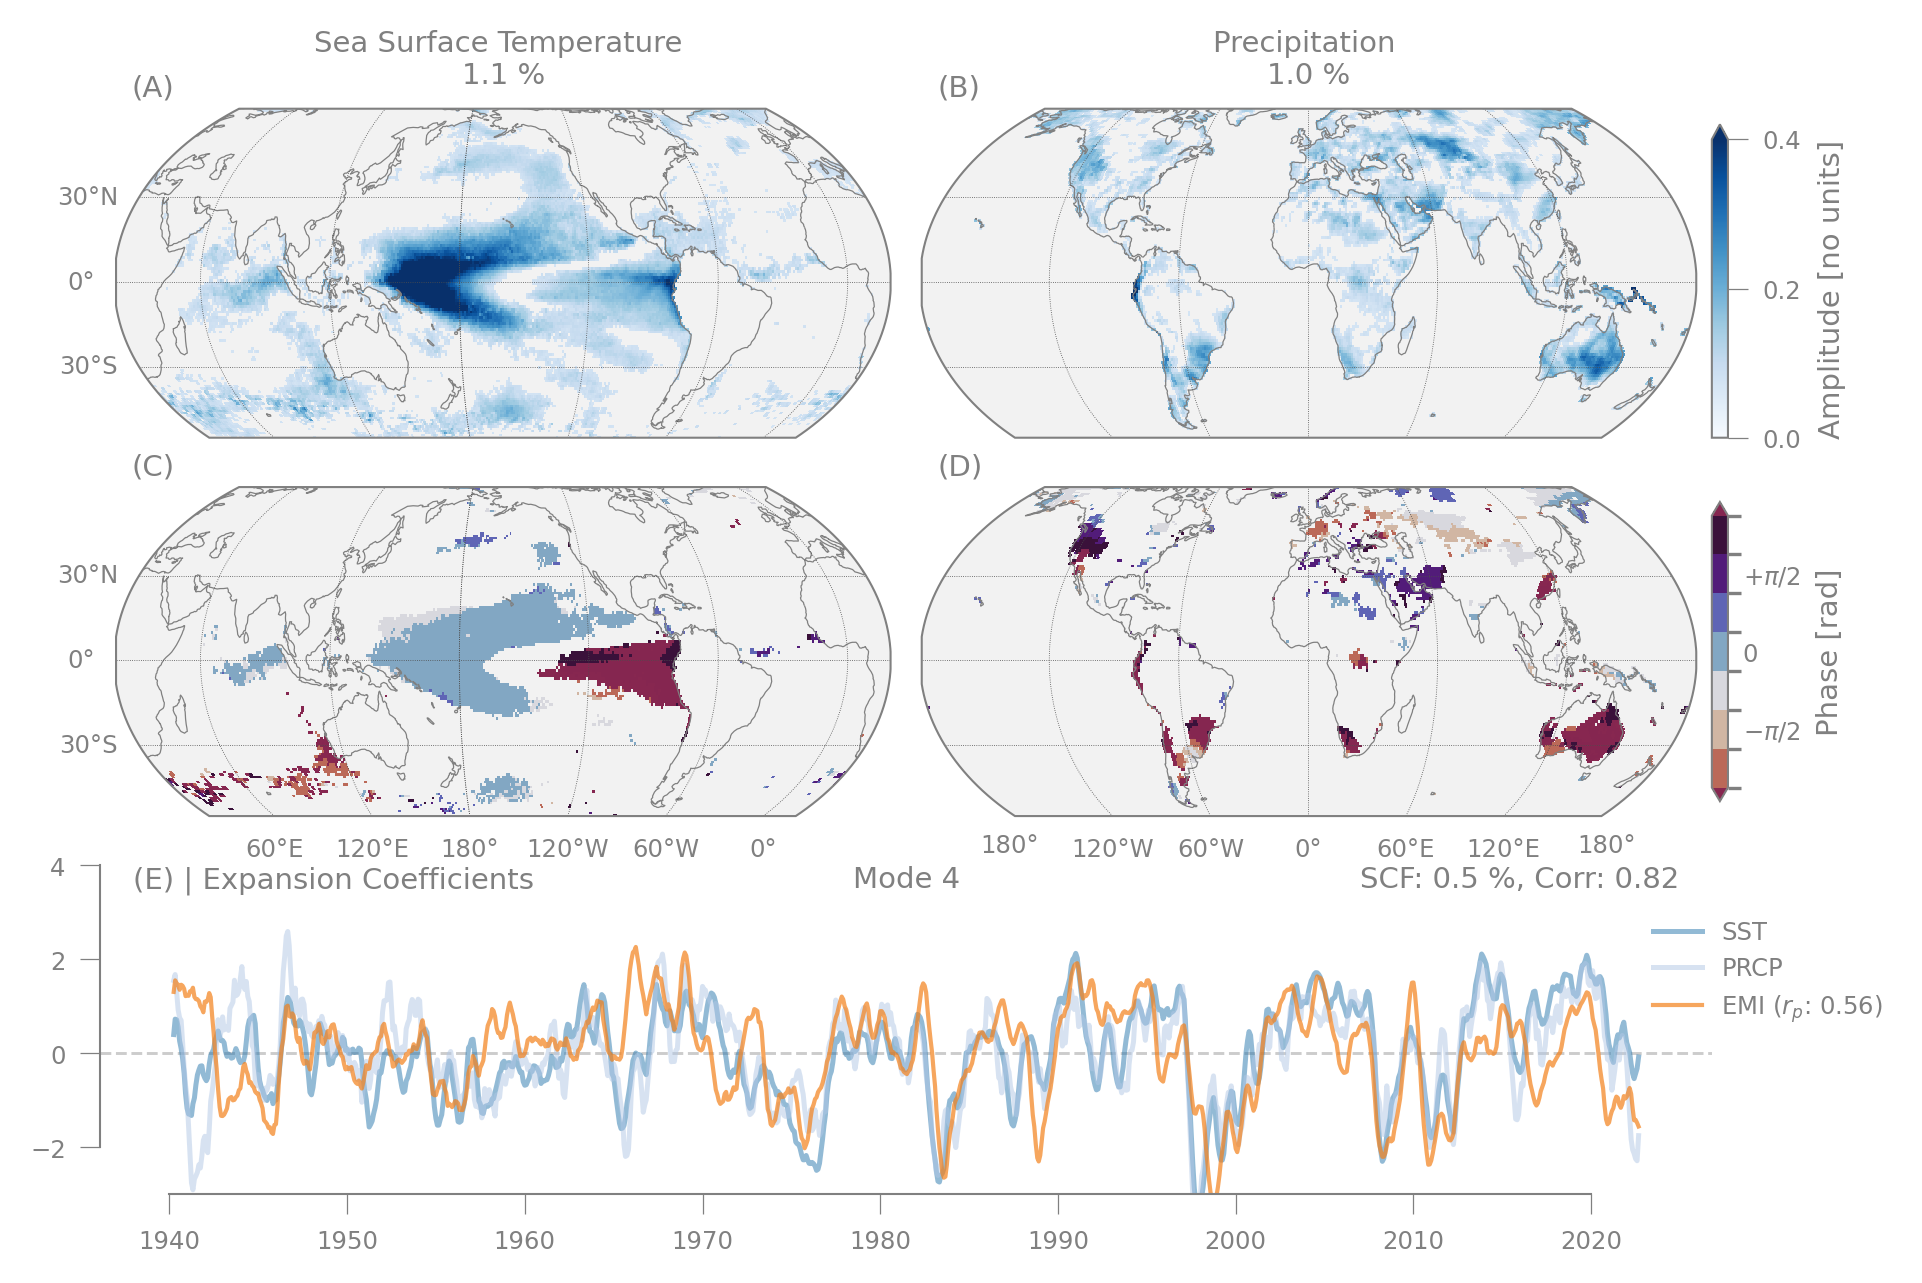
\includegraphics[width=\textwidth]{tele_a100_r22_p1_mode04}
    \caption[Nonlinear ENSO modulation as represented by mode 4 of varimax-rotated Hilbert MCA applied to SST and precipitation.]{\textbf{Nonlinear ENSO modulation as represented by mode 4 of varimax-rotated Hilbert MCA applied to SST and precipitation.} The orange line represents the El Niño Modoki (EMI) index for comparison, along with its Pearson correlation coefficient with the SST expansion coefficients. For more details, refer to the description in Figure~\ref{fig:tele:mode01_a100}.}
    \label{fig:tele:mode04_a100}
\end{figure}


\paragraph{Mode 4---Nonlinear ENSO Modulation} 
Mode 4 describes an oscillating SST anomaly mainly confined to the central Pacific (Figure~\ref{fig:tele:mode04_a100}), resembling the pattern popularized by \citet{ashok_nino_2007} as "El Niño Modoki", represented by the EMI ($\rho_4^{\text{EMI}}=0.56$). This pattern consists of higher SSTs in the central Pacific and lower SSTs in the eastern Pacific, which correlate with reduced precipitation in the East Asian monsoon region \cite{feng_different_2011}, Australia \cite{taschetto_nino_2009}, parts of South America \cite{tedeschi_influences_2013}, and South Africa \cite{ratnam_remote_2014}, and vice versa. Some of these teleconnections have recently been identified through event coincidence analysis \cite{wiedermann_differential_2021}, although our analysis suggests additional significant links to the East Asian monsoon region. Later research by \citet{takahashi_enso_2011}, however, indicated that El Niño Modoki and the classical El Niño are essentially the same phenomenon, and that the perceived differences highlight the dynamic range of the system, specifically the nonlinearity of ENSO. Following this interpretation, the teleconnections identified in our analysis should not be considered a separate mode but rather a modulation of ENSO mode 2 due to the system's nonlinear behavior.

The power spectral density of this ENSO modulation shows a rather broadband energy distribution mostly indistinguishable from the theoretical "red noise" spectrum, with the exception from some periodicities around 18 months (Figure~\ref{fig:tele:psd}~D). In particular, the energy distribution is markedly different from the periodicities typically associated with ENSO (2 to 7 years). Overall, the phase does not provide a clear interpretation apart from zero and $\pm \pi$ phase shifts.

\begin{figure}
    \centering
    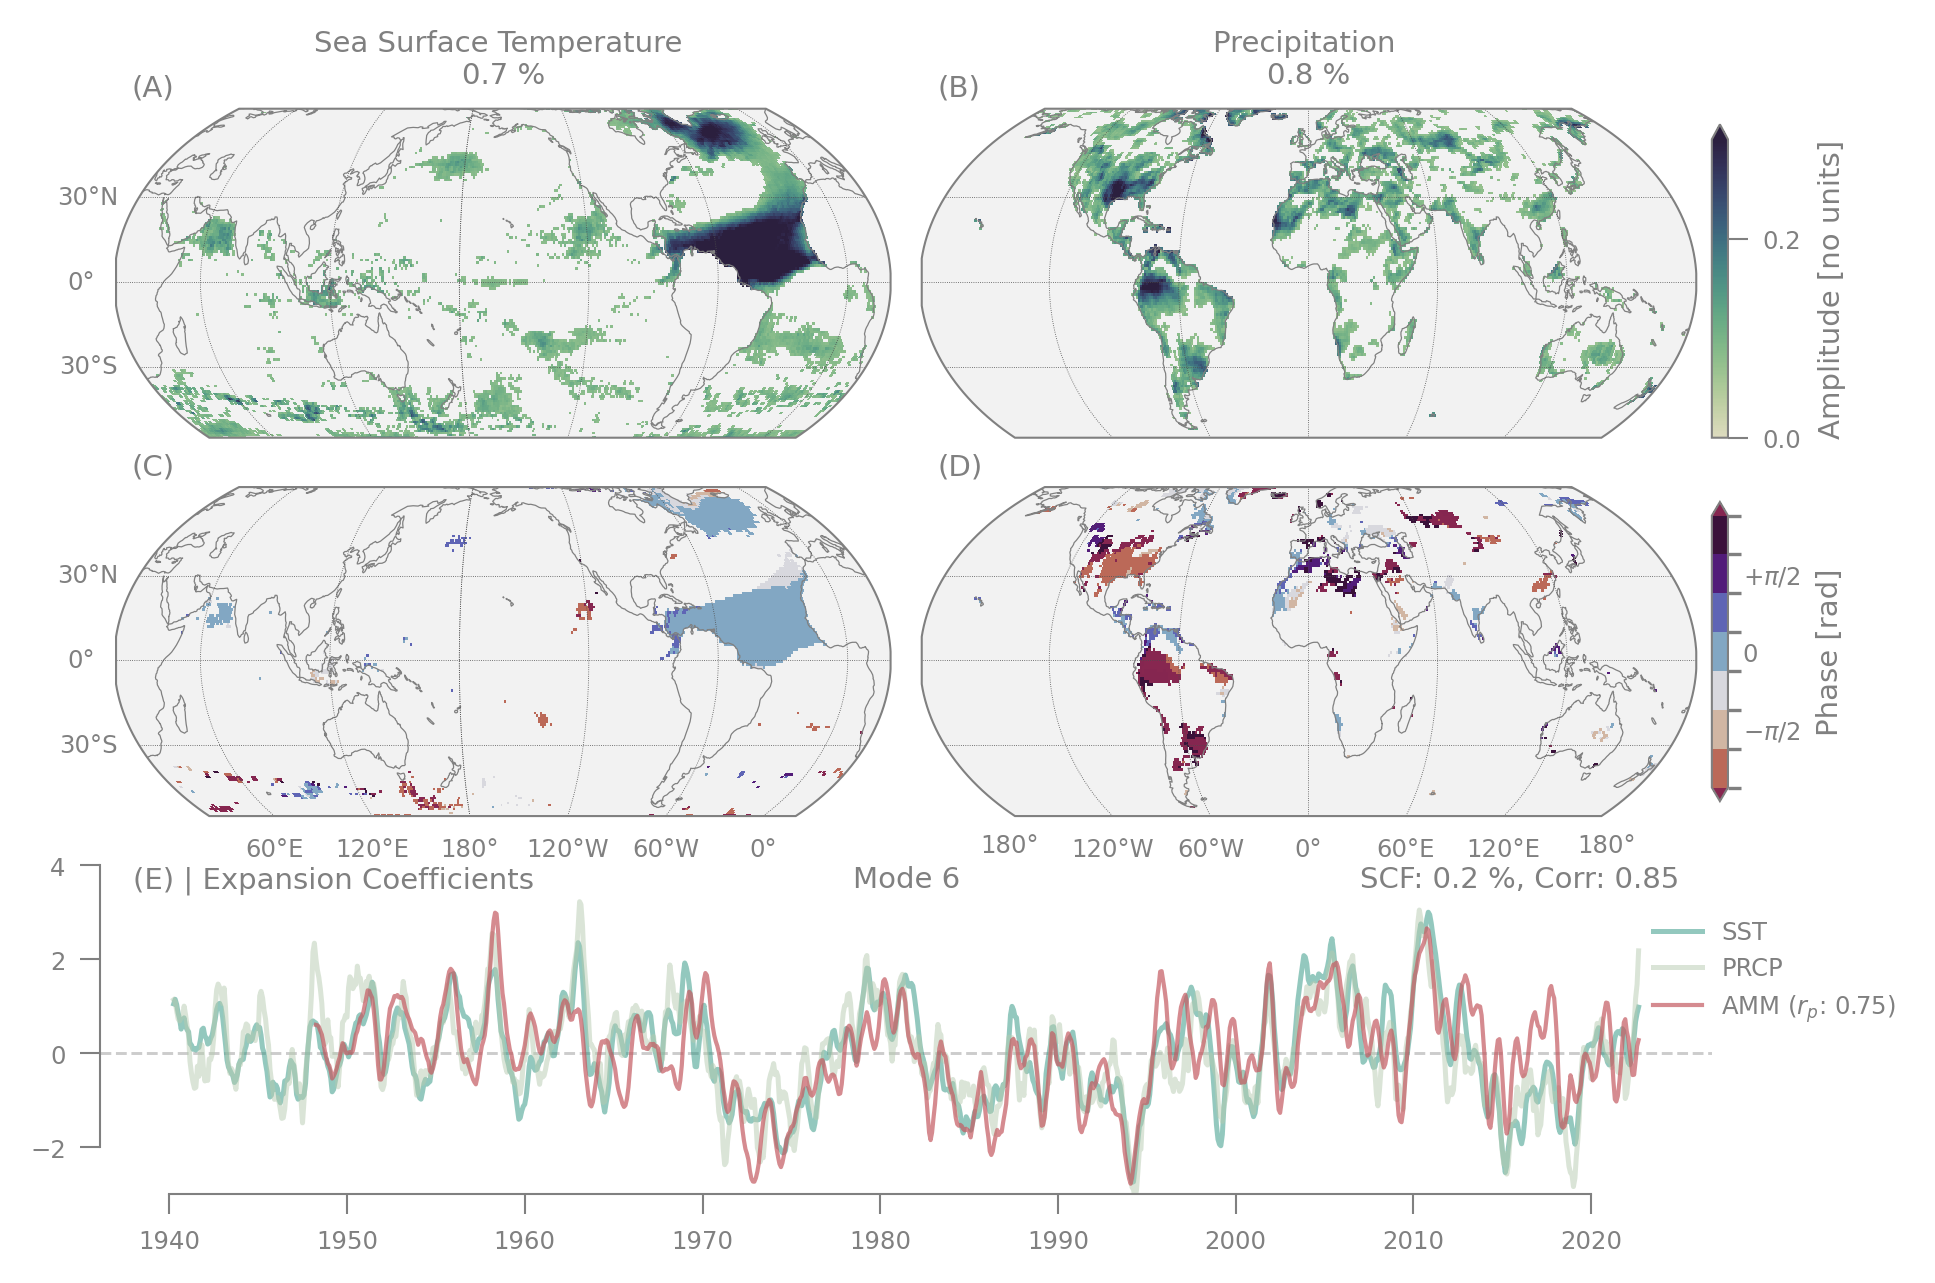
\includegraphics[width=\textwidth]{tele_a100_r22_p1_mode06}
    \caption[Atlantic Meridional Modulation (AMM) as represented by mode 6 of varimax-rotated Hilbert MCA applied to SST and precipitation.]{\textbf{Atlantic Meridional Modulation (AMM) as represented by mode 6 of varimax-rotated Hilbert MCA applied to SST and precipitation.} The orange line represents the AMM index for comparison, along with its Pearson correlation coefficient with the SST expansion coefficients. For more details, refer to the description in Figure~\ref{fig:tele:mode01_a100}.}
    \label{fig:tele:mode06_a100}
\end{figure}

\paragraph{Mode 6---AMM} 
Mode 6 is characterized by an SST pattern concentrated in the tropical and subarctic North Atlantic (Figure~\ref{fig:tele:mode06_a100}), explaining about \qty{0.7}{\percent} of the overall SST variability (Table~\ref{tab:tele:summary}). This pattern represents the AMM, the dominant coupled ocean-atmosphere phenomenon in the tropical Atlantic \cite{servain_relationship_1999}. The AMM's impacts on precipitation---explaining about \qty{0.8}{\percent} of total precipitation variability---in the African Sahel zone, Central America, and northern South America are well documented \cite{lamb_interannual_1986, martin_multidecadal_2014}. Only recently, \citet{vittal_early_2020} found a link between the AMM and Indian summer monsoon rainfall, which they used to improve precipitation forecasts. Additionally, our results suggest further teleconnections between the AMM and precipitation variability over North America, the Mediterranean, and the East Asian monsoon region, offering potential for enhancing local rainfall predictions in these areas. Of particular interest is the southeastern United States, where a phase shift of $-3\pi/4$---corresponding to a time lag of about 9 months assuming a periodicity of 2 years (Figure~\ref{fig:tele:psd}~E)---is observed.


\begin{figure}
    \centering
    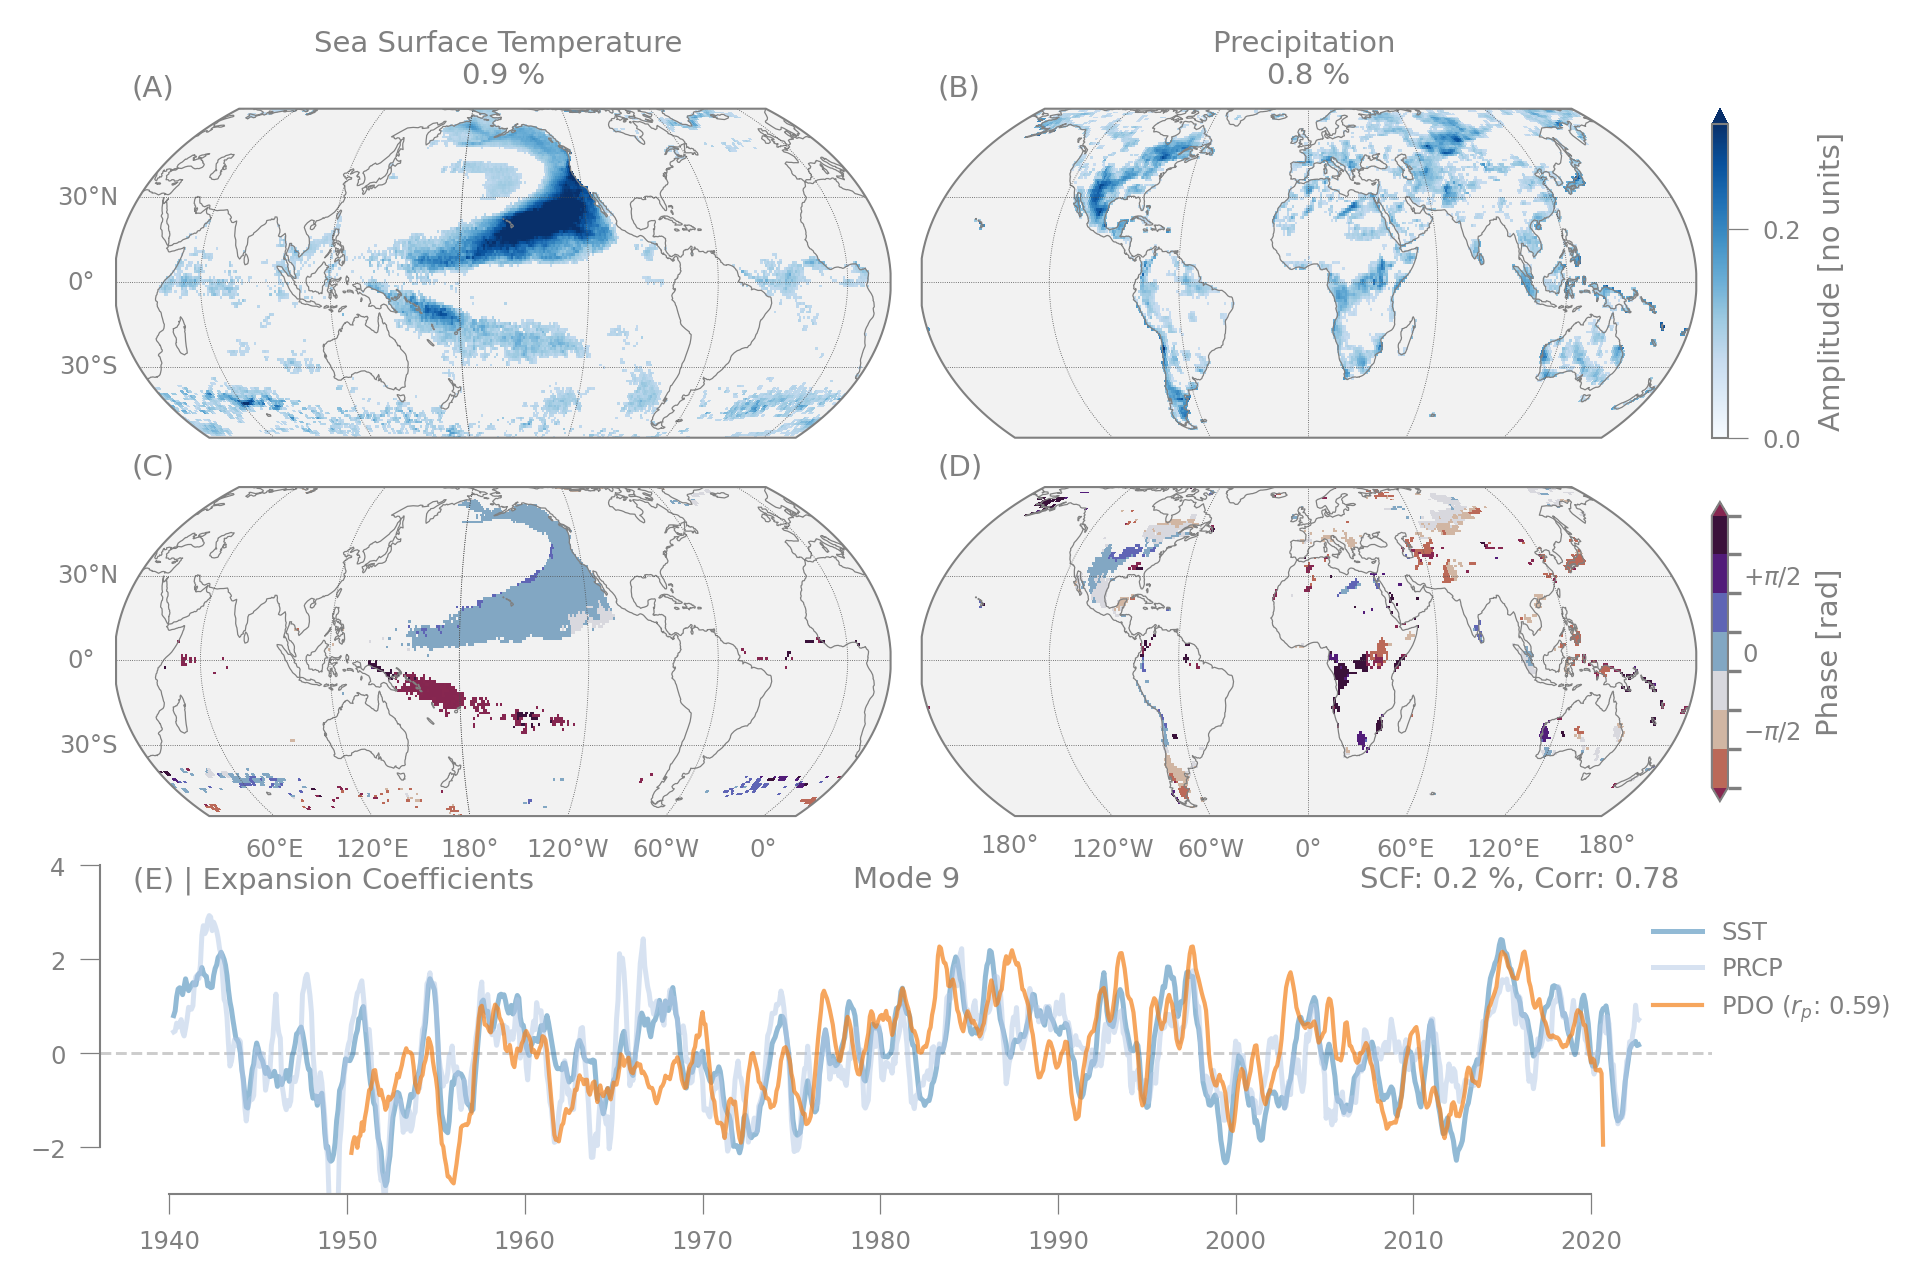
\includegraphics[width=\textwidth]{tele_a100_r22_p1_mode09}
    \caption[Pacific Decadal Oscillation (PDO) as represented by mode 9 of varimax-rotated Hilbert MCA applied to SST and precipitation.]{\textbf{Pacific Decadal Oscillation (PDO) as represented by mode 9 of varimax-rotated Hilbert MCA applied to SST and precipitation.} The orange line represents the PDO index for comparison, along with its Pearson correlation coefficient with the SST expansion coefficients. For more details, refer to the description in Figure~\ref{fig:tele:mode01_a100}.}
    \label{fig:tele:mode09_a100}
\end{figure}


\paragraph{Mode 9---PDO} 
Mode 9 exhibits a slow-oscillating SST pattern in the northeastern Pacific, correlating with localized precipitation patterns distributed across all continents, predominantly in North America (Figures~\ref{fig:tele:mode09_a100}~A,~B). This spatial SST pattern is known as the PDO \cite{mantua_pacific_1997} ($\rho_9^{\text{PDO}}=0.59$), a well-established climate index. Various processes originating in the tropics and extratropics have been proposed as the physical source of the PDO \cite{newman_pacific_2016}, with ENSO and PDO likely responding to the same forcing function \cite{pierce_role_2002}. Our analysis provides a means to disentangle ENSO- and PDO-related precipitation patterns, which are often similar in western North America \cite{hu_interferential_2009}. Typically, the PDO exhibits strong energy around periodicities of 30 years; however, due to our preprocessing (using block sizes of 9 years), we cannot resolve such long periodicities in our analysis. Instead, we find higher-frequency, multi-year periodicities around 4 years (Figure~\ref{fig:tele:psd}~I), likely due to the significant feedbacks between ENSO and PDO modes \cite{mills_seasonal_2013, tang_positive_2024}. This finding is interesting because this spectral peak is not visible in the official PDO index, indicating slight differences in the composition of the PDO mode in our analysis compared to the traditional PDO index.


\begin{figure}
    \centering
    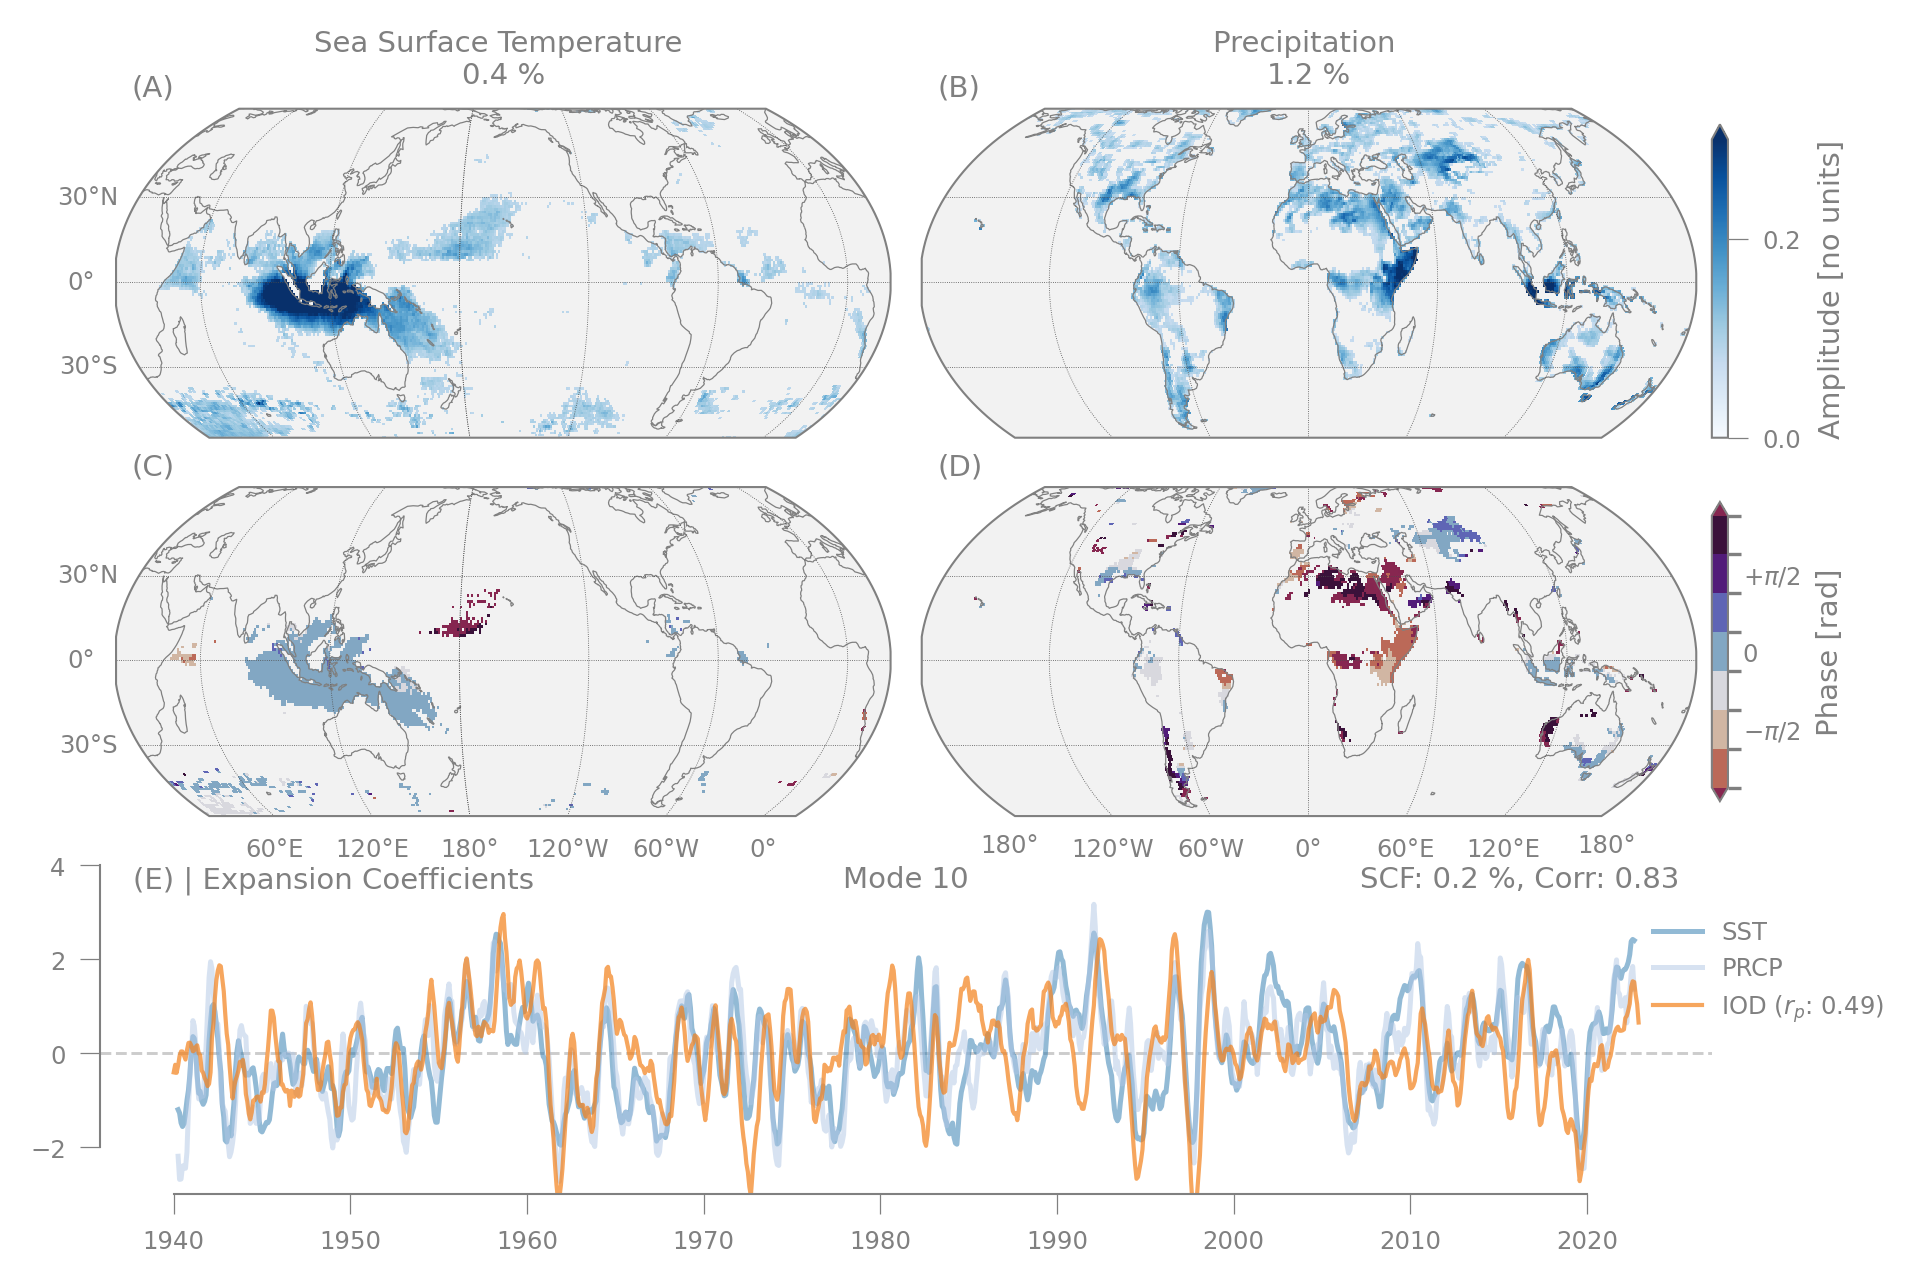
\includegraphics[width=\textwidth]{tele_a100_r22_p1_mode10}
    \caption[Indian Ocean Dipole (IOD) as represented by mode 10 of varimax-rotated Hilbert MCA applied to SST and precipitation.]{\textbf{Indian Ocean Dipole (IOD) as represented by mode 10 of varimax-rotated Hilbert MCA applied to SST and precipitation.} The orange line represents the IOD index for comparison, along with its Pearson correlation coefficient with the SST expansion coefficients. For more details, refer to the description in Figure~\ref{fig:tele:mode01_a100}.}
    \label{fig:tele:mode10_a100}
\end{figure}

\paragraph{Mode 10---IOD} Mode 10 resembles the IOD ($\rho_{10}^{IOD}=0.49$), a coupled ocean-atmosphere phenomenon in the tropical Indian ocean \cite{saji_possible_2003} that explains about \qty{0.4}{\percent} of the total SST variability. The SST pattern is characterized by a dipole structure with higher SST in the western and lower SST in the eastern Indian Ocean. The associated precipitation pattern is mainly concentrated in the surrounding tropical land masses, namely central east Africa and Oceania, explaining \qty{1.2}{\percent} of the total precipitation variability (Figure~\ref{fig:tele:mode10_a100}~A,B). The phase function shows a clear phase shift of $+\pi/2$, i.e. anti-correlation between precipitation patterns around the eastern and western Indian ocean, mirroring the dipole in the tropical Indian SSTs. Note that our results has only a weakly expressed dipole, with a much stronger center of attention in the eastern Indian ocean and much lower amplitude in the western Indian ocean (Figure~\ref{fig:tele:mode10_a100}~C,~D). Although the PSD of this mode shows significant energy around 18-24 months compared to the "red noise" model, the PSD remains relatively flat across a wide range of frequencies, reflecting the aperiodic and irregular nature of the IOD (Figure~\ref{fig:tele:psd}~J).



\paragraph{Other Modes of Shared Variability}
In our previous discussion, we focused on the dominant modes of shared variability identified by \citet{rieger_lagged_2021} using the MCA framework. With the expanded dataset used here, covering a broader spatial and temporal scope, we identified additional modes---specifically modes 5, 7, and 8---that bring new insights worth noting. Here, we provide a brief overview of these modes, pointing to some interesting preliminary observations while leaving detailed analysis for future work.

Mode 5 (Figure~\ref{app:fig:tele:mode05_a100_p1}) closely mirrors aspects of the atmospheric Pacific-South American (PSA) mode, which influences multiscale spatiotemporal patterns in the upper South Pacific Ocean. This mode significantly drives oceanic variability in the South Pacific subtropics, producing a potentially predictable climate signal connected to tropical regions \cite{lou_linking_2021}. This mode shows increased rainfall over southeastern South America, consistent with patterns observed during ENSO events \cite{mo_pacificsouth_2001}, though it does not reflect the typical rainfall deficits in northeastern Brazil associated to the PSA mode  (Figure~\ref{app:fig:tele:mode05_a100_p1}~B,~D).

Mode 7 (Figure~\ref{app:fig:tele:mode07_a100_p1}) reveals a distinct variability pattern in the eastern Indian Ocean, with precipitation teleconnections extending to central Africa and the southeastern United States. This suggests interconnected weather systems across these regions, highlighting the global reach of this mode. 

Mode 8 (Figure~\ref{app:fig:tele:mode08_a100_p1}) is characterized by SST variability primarily north of the Arctic Circle. This mode shows a positive trend combined with slow-frequency fluctuations, indicating a possible link to global warming. Its unique spatial focus may be related to Arctic amplification, where the Arctic region warms faster than the rest of the planet, representing a different, potentially nonlinear aspect of climate variability.

\subsection{Beyond Covariance---Applying the CPCCA Framework}
As outlined in Section~\ref{sec:theory:cpcca}, the CPCCA framework provides a complementary persepctive to MCA by balancing covariance and correlation. The motivation for applying CPCCA is twofold. First, it serves as a robustness check for the teleconnections identified through MCA---if modes consistently emerge across both covariance- and correlation driven approaches, their reliability is reinforced. Second, CPCCA offers a different lens by prioritizing correlation over covariance, potentially uncovering new teleconnections that explain less covariance but exhibit stronger correlations, making them more robust to differing variance scales.

To perform CPCCA, we applied the same preprocessing steps as for Hilbert MCA, including Hilbert transforming the data and conducting an initial PCA reduction using the same number of retained modes. The CPCCA regularization parameters $\alpha_s$, which control the balance between covariance (MCA, $\alpha_s=1$) and correlation (CCA, $\alpha_s=0$), were determined using the objective selection method proposed by \citet{swenson_continuum_2015}, yielding values of \num{0.0011} and \num{0.0013} for SST and precipitation, respectively. These values indicate a strong focus on correlation rather than covariance. To ensure stability in the extracted modes, we used the mode stability index $\kappa$ to determine the optimal number of modes to rotate, resulting in 28 modes. Both orthogonal and oblique rotation were performed, with Figures~\ref{app:fig:tele:mode01_a000_p1}---\ref{app:fig:tele:mode10_a000_p1} and Figures~\ref{app:fig:tele:mode01_a000_p2}---\ref{app:fig:tele:mode10_a000_p2} in the Appendix presenting the first ten modes for each case.

The results from CPCCA confirm that many modes previously identified through MCA reappear, often in different orders but maintaining similar spatial structures. This consistency strengthens confidence in their robustness. Specifically, the seasonal cycle, ENSO, the tropical warming trend, and the AMM persist across both analyses. The PDO and nonlinear ENSO modulations also emerge, though they appear as a single combined mode (Figure~\ref{app:fig:tele:mode04_a000_p1}), highlighting their close dynamical link. While the dominant modes remain stable, CPCCA also reveals additional modes that were not present among the first 10 modes of the MCA result.

One particularly significant result is CPCCA mode 5 (Figure~\ref{app:fig:tele:mode05_a000_p1}), which uncovers a teleconnection linking SST anomalies in the western tropical Pacific to precipitation in Northern Europe---a pattern that was not identified using MCA. The ability of CPCCA to extract this relationship suggests that MCA's emphasis on maximizing variance may obscure physically meaningful, but lower-variance, connections. This finding aligns with \citet{straaten_correcting_2023}, who identified this SST pattern as a predictor for European summer temperatures on sub-seasonal timescales. Our results extend this insight to precipitation predictability, indicating that this source of predictability may also hold value for seasonal precipitation forecasts. Given the increasing need for skillful seasonal precipitation predictions, particularly in mid-latitude regions, further investigation into the robustness and dynamical underpinnings of this mode is warranted.


\section{Conclusions}\label{sec:tele:conclusions}
In this chapter, we investigated the shared variability between SST and continental precipitation to better understand atmospheric teleconnections----patterns that link climate variations across distant regions. Using rotated Hilbert MCA applied to reanalysis data, we decomposed complex, high-dimensional covariability into dominant modes of shared variability. This framework effectively identified well-established climate phenomena, including the seasonal cycle, ENSO, a warming trend, PDO, AMM, NAO, and IOD, reinforcing the validity of our approach. By capturing both the seasonal cycle and lagged teleconnections within a single framework----without the need to explicitly remove the seasonal cycle----this method provides a comprehensive view of global ocean-atmosphere interactions.

The Hilbert-complexified approach proved particularly effective for identifying time-lagged variability and regularly oscillating patterns within narrow frequency bands. The ability to detect multiple established teleconnection patterns in a single analysis highlights its utility as an exploratory tool for analyzing dense climate datasets, especially when no specific hypothesis is predefined. This approach offers a valuable starting point for deriving more targeted hypotheses for further testing.

Beyond these well-established modes, we uncovered additional patterns of shared variability, including mode 5, which resembles the Pacific-South American (PSA) pattern and highlights connections between the South Pacific subtropics and tropical regions. Mode 7 identifies variability in the eastern Indian Ocean with teleconnections to central Africa and the southeastern United States, while mode 8 reveals SST changes north of the Arctic Circle, suggesting links to Arctic amplification and regional impacts of global warming. These findings open up new opportunities for research into less-explored teleconnection patterns.

To provide a complementary perspective, we extended our analysis by incorporating the CPCCA framework \cite{swenson_continuum_2015}, moving towards a focus of maximum correlation instead of covariance. This revealed modes with higher correlations but lower explained variance, offering an alternative view of SST-precipitation interactions. Notably, CPCCA mode 5 uncovered a unique teleconnection linking SST anomalies in the western tropical Pacific to precipitation in northern Europe (Fig.~\ref{app:fig:tele:mode05_a000_p1}), a pattern not captured by MCA but recently identified as a potential source of European summer climate predictability \cite{straaten_correcting_2023}.

Despite its strengths, rotated Hilbert CPCCA has several limitations that should be considered. First, its reliance on covariance/correlation structures means it may not suffice for developing reduced-order dynamical models, which require a deeper understanding of physical mechanisms \cite[e.g.][]{farrell_accurate_2001}. Second, the assumption of linearity in MCA can overlook non-linear ocean-atmosphere interactions, such as those inherent in ENSO, which were captured in multiple modes (Fig.~\ref{fig:tele:mode02_a100}~and~\ref{fig:tele:mode04_a100}). Finally, the method assumes that data can be represented as a sum of narrowband oscillatory modes, limiting its interpretability for irregular oscillatory patterns like the PDO or IOD.

These limitations highlight opportunities for methodological advancements. Employing the continuous Morlet analytic wavelet transform----as proposed by \citet{guilloteau_rotated_2020}----as an alternative to the Hilbert transform may improve the interpretability of phase information, especially when regularized through rotation. Additionally, non-linear approaches, such as kernel-based methods \cite{akaho_kernel_2007} or neural network approximations \cite{asoh_approximation_1994,hsieh_nonlinear_2000}, could help address the non-linearity in teleconnection patterns. However, interpreting the underlying spatial patterns in kernel methods remains challenging due to the pre-image problem. Recent advancements, including linear approximations \cite{bueso_nonlinear_2020} and composite patterns \cite{hannachi_bimodality_2019}, offer potential solutions, making non-linear methods more accessible and interpretable for climate research.

In summary, our study demonstrates that combining varimax-rotated Hilbert extensions with MCA and CPCCA provides a robust framework for identifying and interpreting dominant modes of shared variability between SST and continental precipitation. These methods not only enhance our understanding of atmospheric teleconnections but also uncover new teleconnection patterns with significant potential for improving climate predictions on seasonal to decadal timescales.